
\documentclass[11pt,a4paper]{book}
\usepackage[utf8x]{inputenc}
\usepackage[T1]{fontenc}
\usepackage[spanish]{babel}
\usepackage{amsmath}
\usepackage{amssymb,amsfonts,textcomp}
\usepackage{color}
\usepackage{array}
\usepackage{multirow}
\usepackage{hhline}
\usepackage{hyperref}
\usepackage{float}
\usepackage{xkeyval}
\usepackage[pdftex]{graphicx}
\usepackage[yyyymmdd,hhmmss]{datetime}
\usepackage[usenames,dvipsnames]{xcolor}
\usepackage{appendix}
\usepackage{listings}
\usepackage{enumitem}
\usepackage{fancyvrb}


\usepackage{amsthm} %load after amsmath

\newtheoremstyle{ejemplo}% hname
{11pt}% Space above
{3pt}% Space below
{\footnotesize}% Body font
{}% Indent amount
{\bfseries}% Theorem head font
{}% Punctuation after theorem head
{\newline}% Space after theorem head
{}% Theorem head spec (can be left empty, meaning ‘normal’)

\theoremstyle{ejemplo}
\newtheorem{ejemplo}{Ejemplo}[section]


\usepackage{multicol}


%\usepackage{wasysym}
\definecolor{dkgreen}{rgb}{0,0.6,0}
\definecolor{gray}{rgb}{0.5,0.5,0.5}
\definecolor{mauve}{rgb}{0.58,0,0.82}
\definecolor{lstbackground}{rgb}{0.95,0.95,0.95}
\definecolor{white}{rgb}{100,100,100}
% \lstset{frame=tb,
% 	backgroundcolor=\color{lstbackground},
%   language=Bash,
%   aboveskip=3mm,
%   belowskip=3mm,
%   showstringspaces=false,
%   columns=flexible,
%   basicstyle={\small\ttfamily},
%   numbers=none,
%   numberstyle=\tiny\color{gray},
%   keywordstyle=\color{blue},
%   %commentstyle=\color{dkgreen},
%   stringstyle=\color{mauve},
%   breaklines=true,
%   breakatwhitespace=true,
%   extendedchars=true,
%   tabsize=3
% }
\lstset{
  backgroundcolor=\color{lstbackground},
% language=Bash,
  aboveskip=3mm,
  belowskip=3mm,
  showstringspaces=false,
  columns=flexible,
  basicstyle={\small\ttfamily\bfseries},
  numbers=none,
%  xleftmargin=0.5cm,
%  xrightmargin=0.5cm,
%  frame=lr,framesep=0.5cm,framerule=0pt,
%  numberstyle=\tiny\color{gray},
%  keywordstyle=\color{blue},
%  commentstyle=\color{dkgreen},
%  stringstyle=\color{mauve},
  breaklines=true,
  breakatwhitespace=true,
  tabsize=4
}

% \lstnewenvironment{codecell}
%   	{\lstset{
% 	  aboveskip=3mm,
% 	  belowskip=3mm,
% 	  showstringspaces=false,
% 	  columns=flexible,
% 	  basicstyle={\small\ttfamily},
% 	  numbers=none,
% 	  breaklines=true,
% 	  breakatwhitespace=true,
% 	  tabsize=4
% 	  }
% 	} {}
% 

\lstnewenvironment{mylistings}
  {\lstset{language=C++,
    backgroundcolor=\color{listingscolor}, % set backgroundcolor
    basicstyle=\footnotesize,% basic font setting
    }%
  }
  {}

\lstnewenvironment{codecell}
  {\lstset{basicstyle={\small\ttfamily},% basic font setting
    backgroundcolor=\color{white}}%
  }
  {}



\usepackage[font=small,skip=1cm]{caption}

%\DeclareCaptionFont{black}{ \color{black} }
%\DeclareCaptionFormat{listing}{
%  \colorbox[cmyk]{0.93, 0.95, 0.95,0.01 }{
%    \parbox{\textwidth}{\hspace{15pt}#1#2#3}
%  }
%}
%\captionsetup[lstlisting]{ format=listing, labelfont=black, textfont=black, singlelinecheck=false, margin=0pt, font={bf,footnotesize} }
%\captionsetup[lstlisting]{format=plain, font={footnotesize}}
%\captionsetup[figure]{format=plain,font={footnotesize}}
% ...


%\renewcommand{\lstlistingname}{Code}
\usepackage{verbatim}

%\addto\captionsspanish {%
%	\def\appendixname{Apéndices}
%}
% Outline numbering
\setcounter{secnumdepth}{1}
% Reset section numbering between parts
\makeatletter
\@addtoreset{section}{chapter}
\makeatother  
% List styles
\newcommand\liststyleLi{%
\renewcommand\labelitemi{\tiny${\blacksquare}$}
\renewcommand\labelitemii{\tiny${\square}$}
\renewcommand\labelitemiii{\tiny${\circ}$}
\renewcommand\labelitemiv{\tiny${\circ}$}
}
\newcommand\liststyleLii{%
\renewcommand\labelitemi{{\textbullet}}
\renewcommand\labelitemii{${\circ}$}
\renewcommand\labelitemiii{${\blacksquare}$}
\renewcommand\labelitemiv{{\textbullet}}
}
\newcommand\liststyleLiii{%
\renewcommand\labelitemi{{\textbullet}}
\renewcommand\labelitemii{${\circ}$}
\renewcommand\labelitemiii{${\blacksquare}$}
\renewcommand\labelitemiv{{\textbullet}}
}

\liststyleLi

% Page layout (geometry)
\setlength\voffset{-1in}
\setlength\hoffset{-1in}
\setlength\topmargin{2cm}
\setlength\oddsidemargin{2cm}
\setlength\textheight{23.246668cm}
\setlength\textwidth{17.006cm}
\setlength\footskip{26.144882pt}
\setlength\headheight{1.016cm}
\setlength\headsep{0.508cm}
% Footnote rule
\setlength{\skip\footins}{0.119cm}
\renewcommand\footnoterule{\vspace*{-0.018cm}\setlength\leftskip{0pt}\setlength\rightskip{0pt plus 1fil}\noindent\textcolor{black}{\rule{0.25\columnwidth}{0.018cm}}\vspace*{0.101cm}}
% Pages styles
\makeatletter
\newcommand\ps@Standard{
  \renewcommand\@oddhead{{\raggedleft Cabecera \ } {\raggedright \thepage{}}}
  \renewcommand\@evenhead{\@oddhead}
  \renewcommand\@oddfoot{}
  \renewcommand\@evenfoot{\@oddfoot}
  \renewcommand\thepage{\arabic{page}}
}

% \pagestyle{Standard}
\usepackage{fancyhdr}
\pagestyle{fancy}


%%--------------------------------------
% F O N T S 
% \usepackage{dejavu}
%\usepackage{librebaskerville}
%\usepackage{sans}
%\usepackage{libertine}
%\usepackage{lmodern}
%\usepackage{opensans}
%\usepackage{helvet}
%\usepackage{times}

\usepackage{lmodern}
\renewcommand*\familydefault{\sfdefault} %% Only if the base font of the document is to be sans serif


%% LaTeX Preamble - Font choices
%% Each block selects new math, roman (serif), sans serif, and typewriter fonts.
%% Delete or comment out all but one to make your choice.

% Fourier for math | Utopia (scaled) for rm | Helvetica for ss | Latin Modern for tt
%\usepackage{fourier} % math & rm
%\usepackage[scaled=0.875]{helvet} % ss
%\renewcommand{\ttdefault}{lmtt} %tt

% Latin Modern (similar to CM with more characters)
%\usepackage{lmodern} % math, rm, ss, tt
%\usepackage[T1]{fontenc}

% Palatino for rm and math | Helvetica for ss | Courier for tt
%\usepackage{mathpazo} % math & rm
%\linespread{1.05}        % Palatino needs more leading (space between lines)
%\usepackage[scaled]{helvet} % ss
%\usepackage{courier} % tt
%\normalfont
%\usepackage[T1]{fontenc}

% Euler for math | Palatino for rm | Helvetica for ss | Courier for tt
%\renewcommand{\rmdefault}{ppl} % rm
%\linespread{1.05}        % Palatino needs more leading
%\usepackage[scaled]{helvet} % ss
%\usepackage{courier} % tt
%\usepackage{euler} % math
%\usepackage{eulervm} % a better implementation of the euler package (not in gwTeX)

%\normalfont
%\usepackage[T1]{fontenc}

% Times for rm and math | Helvetica for ss | Courier for tt
%\usepackage{mathptmx} % rm & math
%\usepackage[scaled=0.90]{helvet} % ss
%\usepackage{courier} % tt
%\normalfont
%\usepackage[T1]{fontenc}

% !! COMMERICAL FONT !! Lucida Bright (w/expert package)
%\usepackage[T1]{fontenc}
%\usepackage[expert,vargreek,altbullet]{lucidabr}

%% END Font choices
%%---------------------------------------------
% \renewcommand*\familydefault{\sfdefault}
% \pagestyle{Standard}
\usepackage{mdframed}


% footnotes configuration
\makeatletter
\renewcommand\thefootnote{\arabic{footnote}}
\makeatother
\usepackage{graphicx}

\usepackage{xkeyval}
\usepackage{pifont}
\usepackage{xcolor}
\newcommand{\revisar}[1]{{\color{red}[#1]}}
%\newcommand{\nota}[1]{{\color{red}[#1]}}
%\newcommand{\revisar}[1]{}

\newcommand{\borrador}{
\revisar{\today, \currenttime  -  Material en preparación, se ruega no imprimir mientras aparezca esta nota}
}




\newcommand{\nota}[1]{}

\newcommand{\nonota}[1]{#1}

\newcommand{\quotes}[1]{``#1''}

   
\newcommand{\shade}[1]{\textcolor{black!50}{#1}}

% ancho opcional, por defecto 15cm
% \figura{copyleft}{Símbolo de Copyleft}{copyleft.png}
% \figura[6]{copyleft}{Símbolo de Copyleft}{copyleft.png}
\newcommand{\figura}[4][15]{
 \begin{figure}[htb] 
 \centering 
 \includegraphics[width=#1cm]{./img/#4}
 \caption{#3}
 \label{fig:#2} 
 \end{figure} 
}



% tabla{label}{caption}{columns}{contents}
\newcommand{\tabla}[4]{
 \begin{table} 
 \centering 
 \small
 \begin{tabular}{#3}
 #4
 \end{tabular}
 \caption{#2}
 \label{tab:#1} 
 \end{table} 
}

\usepackage{sectsty}
%\usepackage[compact]{titlesec} 
\definecolor{bl}{rgb}{0.0,0.2,0.6} 
\allsectionsfont{\color{bl}\scshape\selectfont}


\newcommand{\recuadro}[1]{
\begin{minipage}[c]{0.84\textwidth}
\begin{mdframed}
#1
\end{mdframed}
\end{minipage}
}

\newcommand{\code}[1]{\lstinline$#1$}

%\usepackage{C}
%\clearpage\clearpage\setcounter{page}{1}\pagestyle{HTML}

\hypersetup{
	colorlinks=true, 
	linkcolor=blue, 
	citecolor=blue, 
	filecolor=blue, 
	urlcolor=blue, 
	pdftitle={Taller de Lenguaje C}, 
	pdfauthor={Eduardo Grosclaude}, 
	pdfsubject={Taller de Lenguaje C para Ciencias de la Computación 2015}, 
	pdfkeywords={Lenguaje C, Taller de programación, Universidad Nacional del Comahue}
}
\title{Taller de Lenguaje C}
\author{Eduardo Grosclaude}
\date{2014-12-09}

% --------------------------------------------------------------------


\begin{document}
\maketitle

\borrador

\newpage
\tableofcontents


\chapter{Introducción al Lenguaje C}


El lenguaje de programación C fue creado por \textbf{Dennis Ritchie} en 1972 en
Bell Telephone Laboratories, con el objetivo de reescribir un sistema
operativo, el UNIX, en un lenguaje de alto nivel, para poder adaptarlo
(es decir, \textit{portarlo}) a diferentes arquitecturas. Por este motivo sus
creadores se propusieron metas de diseño especiales, tales como: 

\begin{itemize}
\item Poder utilizar todos los recursos del hardware (\quotes{acceso al bajo nivel}). 
\item Obtener código generado eficiente en uso de memoria y en tiempo de ejecución (programas pequeños y veloces).
\item Compilador portable (implementable en cualquier arquitectura).
\end{itemize}


Actualmente existen implementaciones de C para todas las arquitecturas y
sistemas operativos, y es el lenguaje más utilizado para la
\textbf{programación de sistemas}. Por su gran eficiencia resulta ideal para
la programación de \textbf{sistemas operativos}, \textbf{drivers de dispositivos},
\textbf{herramientas de programación}. El 95\% del sistema operativo UNIX
está escrito en C, así como gran parte de los modernos
sistemas y ambientes operativos, y los programas de administración o aplicación que corren
sobre ellos.

%TODO
%\href{info/info1.html#info1}{Mas información ...} 

\section{Características del lenguaje}
C es un lenguaje compilado. A nivel sintáctico, presenta grandes
similitudes formales con Pascal, pero las diferencias entre ambos son
importantes. A pesar de permitir \textbf{operaciones de bajo nivel}, tiene las
\textbf{estructuras de control}, y permite la \textbf{estructuración de datos}, propias
de los lenguajes procedurales de alto nivel. 

Un programa en C es, por lo general, más \textbf{sintético} que en otros
lenguajes procedurales; la idea central que atraviesa todo
el lenguaje es la minimalidad. La definición del lenguaje consta de
muy pocos elementos, y tiene muy pocas \textbf{palabras reservadas}. Como rasgo
distintivo, en C no existen, rigurosamente hablando, funciones o
procedimientos de uso general del programador. Por ejemplo, \textbf{no tiene
funciones de entrada/salida}; la definición del lenguaje apenas
alcanza a \textbf{las estructuras de control y los operadores}. La idea de
definir un lenguaje sin funciones es, por un lado, hacer posible que el
compilador sea \textbf{pequeño, fácil de escribir e inmediatamente
portable}; y por otro, permitir que sea el usuario quien defina sus
propias funciones cuando el problema de programación a resolver tenga
requerimientos especiales. 

Sin embargo, se ha establecido un conjunto mínimo de funciones,
llamado la \textbf{Biblioteca Standard} del lenguaje C, que todos los
compiladores proveen, a veces con agregados. La filosofía de la
Biblioteca Standard es la portabilidad, es decir, casi no incluye
funciones que sean específicas de un sistema operativo determinado.
Aquellas que sí incluye están orientadas a la programación de sistemas, y a
veces no resultan suficientes para el programador de aplicaciones. No
provee, por ejemplo, la capacidad de manejo de archivos indexados, ni
funciones de entrada/salida interactiva por consola que sean seguras
(\quotes{a prueba de usuarios}). Esta deficiencia
se remedia utilizando bibliotecas de funciones \quotes{de
terceras partes} (creadas por el usuario u obtenidas de
otros programadores). 

El usuario puede escribir sus propios procedimientos (llamados
\textbf{funciones} aunque no devuelvan valores). Aunque existe la
noción de \textbf{bloque} de sentencias (sentencias encerradas entre llaves), el lenguaje se dice \textbf{\textit{no}
estructurado en bloques} porque no pueden definirse funciones dentro de
otras. Las funciones de la Biblioteca Standard no tienen ningún
privilegio sobre las del usuario y \textbf{sus nombres no son palabras
reservadas}; el usuario puede reemplazarlas por sus propias funciones
simplemente dándoles el mismo nombre. 

El lenguaje entrega completamente el control de la máquina subyacente
al programador, no realizando controles de tiempo de ejecución. Es
decir, no verifica condiciones de error comunes como \textbf{\textit{overflow}
de variables}, \textbf{errores de entrada/salida}, o \textbf{consistencia de argumentos}
en llamadas a funciones. Como resultado, es frecuente que el
principiante, y aun el experto, cometan errores de programación que
no se hacen evidentes enseguida, ocasionando problemas y costos de
desarrollo. Permite una gran libertad sintáctica al programador. No
es fuertemente tipado. Cuando es necesario, se realizan \textbf{conversiones
automáticas de tipo} en las asignaciones, a veces \textbf{con efectos
laterales inconvenientes} si no se tiene precaución. Una función que
recibe determinados parámetros formales puede ser invocada con
argumentos reales de otro tipo. 

Se ha dicho que estas características
\quotes{liberales} posibilitan la realización de
proyectos complejos con más facilidad que otros lenguajes como Pascal
o Ada, más estrictos; aunque al mismo tiempo, así resulta más
difícil detectar errores de programación en tiempo de
compilación. En este sentido, según los partidarios de la
tipificación estricta, C no es un buen lenguaje. Gran parte del
esfuerzo de desarrollo del estándar ANSI se dedicó a dotar al C de
elementos para mejorar esta deficiencia. 

Los \textbf{tipos de datos} no tienen un tamaño determinado por la definición
del lenguaje, sino que diferentes implementaciones pueden adoptar
diferentes convenciones. Paradójicamente, esta característica
obedece al objetivo de lograr la \textbf{portabilidad} de los programas en C. El
programador está obligado a no hacer ninguna suposición sobre los
tamaños de los objetos de datos, ya que lo contrario haría al
software dependiente de una arquitectura determinada (\quotes{no portable}). 

Una característica especial del lenguaje C es que el \textbf{pasaje de
argumentos a funciones} se realiza siempre \textbf{por valor}. ¿Qué ocurre
cuando una función debe \textbf{modificar} datos que recibe como
argumentos? La única salida es pasarle -por valor- la dirección del
dato a modificar. Las consecuencias de este hecho son más fuertes de
lo que parece a primera vista, ya que surge la necesidad de todo un
conjunto de técnicas de \textbf{manejo de punteros} que no siempre son bien
comprendidas por los programadores poco experimentados, y abre la
puerta a sutiles y escurridizos errores de programación. Quizás
este punto, junto con el de la ausencia de chequeos en tiempo de
ejecución, sean los que le dan al C fama de \quotes{difícil
de aprender}. 

Por último, el C \textbf{no es un lenguaje orientado a objetos}, sino que
adhiere al paradigma tradicional de \textbf{programación procedural}. No
soporta la orientación a objetos propiamente dicha, al no
proporcionar herramientas fundamentales, como la herencia. Sin embargo,
algunas características del lenguaje permiten que un proyecto de
programación se beneficie de todas maneras con la aplicación de
algunos principios de la orientación a objetos, tales como el
ocultamiento de información y el encapsulamiento de
responsabilidades. El lenguaje C++, orientado a objetos, \textbf{no }es
una versión más avanzada del lenguaje o un compilador de C con
más capacidades, sino que \textbf{se trata de un lenguaje completamente
diferente}. 

\section{Evolución del lenguaje}
La primera definición oficial del lenguaje fue dada en 1978 por
\textbf{Brian Kernighan y Dennis Ritchie} (Fig. \ref{fig:kandr}) en su libro \textbf{El
lenguaje de programación C}. Este lenguaje fue llamado
\textbf{C K\&R}, por las iniciales de sus autores. En 1983 se creó el comité
ANSI para el lenguaje, que en 1988 estableció el estándar ANSI C, con algunas reformas
sobre el C K\&R. Simultáneamente, Kernighan y Ritchie publicaron la
segunda edición de su libro, describiendo la mayor parte de las
características del ANSI C. 


 \begin{figure}[htbp] 
 \centering 
 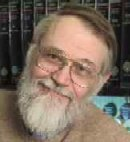
\includegraphics[width=3.44cm,height=3.969cm]{./img/kernighan.jpg} 
 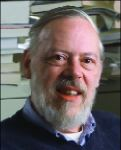
\includegraphics[width=3.44cm,height=3.969cm]{./img/dennis_ritchie.jpg} 
 \caption{Brian Kernighan y Dennis Ritchie, los creadores del lenguaje C} 
 \label{fig:kandr} 
 \end{figure} 


Algunas nuevas características de C99 son: 

\begin{itemize}
\item Matrices de tamaño variable 
\item Soporte de números complejos 
\item Tipos \texttt{long long int} y \texttt{unsigned long long int} de al menos 64 bits 
\item Familia de funciones \texttt{vscanf()} 
\item Comentarios al estilo de C++ prefijando las líneas con la secuencia \texttt{//}. 
\item Familia de funciones \texttt{snprintf()} 
\item Tipo boolean
\end{itemize}


\section{El ciclo de compilación}
Las herramientas esenciales de un ambiente de desarrollo, además de
cualquier \textbf{editor de textos}, son el \textbf{compilador}, el \textbf{vinculador}, 
\textbf{linkeditor} o \textit{linker}, y el \textbf{bibliotecario}. A
estas herramientas básicas se agregan otras, útiles para
automatizar la compilación de proyectos extensos, almacenar y
recuperar versiones de programas fuente, comprobar sintaxis en forma
previa a la compilación, etc. Según el ambiente operativo y
producto de software de que se trate, estas herramientas pueden ser comandos de línea independientes, con
salidas de texto simples, o encontrarse integradas en una interfaz de usuario uniforme, en modo
texto o modo gráfico. 

Cuando encontramos varias de estas herramientas integradas en una sola aplicación, decimos que se trata de un \textbf{IDE} (\textit{Integrated Development Environment}) o ambiente de desarrollo integrado. Un IDE oculta el ciclo de compilación al usuario, con la intención de simplificar el proceso de desarrollo. Sin embargo, conviene conocer qué función se cumple, y qué producto se espera, en cada fase del ciclo de compilación, para poder interpretar las diferentes situaciones de error y poder corregirlas.

\figura[12]{ciclo}{El ciclo de compilación produce un ejecutable \\a partir de archivos fuente.}{ciclo.eps}

\subsection{Compilador}
\begin{itemize}
	\item El compilador acepta un archivo \textbf{fuente}, posiblemente relacionado con
otros (una \textbf{unidad de traducción}), y genera con él un
\textbf{módulo objeto}. Este módulo objeto contiene porciones de
código ejecutable mezclado con \textbf{referencias}, aún no resueltas, a
variables o funciones cuya definición no figura en los fuentes de
entrada. Estas referencias quedan en forma simbólica en el módulo
objeto hasta que se resuelvan en un paso posterior. 
\item Si ocurren errores en esta fase, se deberán a problemas de sintaxis (el código escrito por el programador no respeta la definición del lenguaje).
\end{itemize}

\subsection{Vinculador, linkeditor o \textit{linker}}
\begin{itemize}
\item El vinculador recibe como entrada un conjunto de módulos objeto y
busca \textbf{resolver}, vincular, o enlazar, las referencias simbólicas en ellos,
buscando la definición de las variables o funciones faltantes en los
mismos objetos o en bibliotecas. Éstas pueden ser la Biblioteca
Standard, u otras provistas por el usuario. Cuando el linker encuentra la
definición de un objeto buscado (es decir, de una variable o
función), la copia en el archivo resultante de salida (la
\textit{resuelve}). El objetivo del linker es resolver todas las
referencias pendientes para producir un programa ejecutable. 
\item Si ocurren errores en esta fase, se deberán a que existen variables o funciones cuya definición no ha sido dada (no se encuentran en las unidades de traducción procesadas, ni en ninguna biblioteca conocida por el linker).
\end{itemize}

\subsection{Bibliotecario}
\begin{itemize}
	\item El bibliotecario es un administrador de módulos objeto. Su función
es reunir módulos objeto en archivos llamados \textbf{bibliotecas}, y luego
permitir la extracción, borrado, reemplazo y agregado de módulos.
El conjunto de módulos en una biblioteca se completa con una tabla de
información sobre sus contenidos para que el linker pueda encontrar
rápidamente aquellos módulos donde se ha definido una variable o
función, y así extraerlos durante el proceso de linkedición. 
\item El bibliotecario es utilizado por el usuario cuando desea mantener sus
propias bibliotecas. La creación de bibliotecas propias del usuario
ahorra tiempo de compilación y permite la distribución de software
sin revelar la forma en que se han escrito los fuentes y
protegiéndolo de modificaciones. 
\end{itemize}

Una vez que el código ha sido compilado y vinculado, obtenemos un programa ejecutable. Los errores que pueden producirse en la ejecución ya no corresponden a problemas de compilación, sino que se deben a aspectos de diseño del programa que deben ser corregidos por el programador.

\section{Un primer ejemplo}

El clásico ejemplo de todas las introducciones al lenguaje C es un programa llamado \quotes{\textbf{Hello, World!}}.

\begin{lstlisting}
#include <stdio.h>
/* El primer programa! */
main()
{
	printf("Hola, gente!\n");
}
\end{lstlisting}

\subsection{Funcionamiento del programa}

\begin{itemize}
\item Este programa minimal comienza con una \textbf{directiva de preprocesador} que indica incluir en la unidad de traducción al
archivo de cabecera o \textit{header} \textbf{stdio.h}. Éste contiene, entre otras
cosas, la declaración (o \textbf{prototipo}) de la función de
salida de caracteres \textbf{printf()}, perteneciente a la Biblioteca Standard. Los prototipos se incluyen para
advertir al compilador de los tipos de las funciones y de sus
argumentos. 
\item Entre los pares de caracteres especiales \textbf{/*} y \textbf{*/}se puede insertar cualquier cantidad de líneas de comentarios. 
\item La función \textbf{main()} es el cuerpo principal del programa
(es por donde comenzará la ejecución). Todas las funciones en C están delimitadas por un par de llaves. Terminada la ejecución de
main(), terminará el programa. 
\item La función \texttt{printf()} imprimirá la cadena entre comillas, que es
una \textbf{constante string} terminada por un carácter de
\textbf{nueva línea} (la secuencia especial \quotes{\texttt{{\textbackslash}n}}). 
\end{itemize}

\subsection{Compilación del programa}
Para ver el primer ejemplo en C en funcionamiento:

\begin{enumerate}
	\item Copiar el programa con cualquier editor de textos y guardarlo en un archivo llamado \texttt{hola.c} en el directorio de trabajo del usuario.
	\item Sin cambiar de directorio, invocar al compilador ejecutando el comando \lstinline{gcc hola.c -o hola}. Por defecto, el compilador \textbf{gcc} invocará al vinculador \textbf{ld} para generar el ejecutable a partir del archivo objeto intermedio generado. 
	\item Ejecutar el programa con el comando \lstinline{./hola}. 
\end{enumerate}

Notar el \textit{punto y barra} del principio al ejecutar el programa. El punto y barra le indican al \textbf{shell} que debe buscar el programa en el directorio activo.

Lo mismo, pero de otra manera: 

\begin{enumerate}
	\item Como antes, copiar el programa, o usar el mismo archivo fuente de hace un momento.
	\item Sin cambiar de directorio, ejecutar el comando \lstinline{make hola} en una consola o terminal.
	\item Ejecutar el programa con el comando \lstinline{./hola}. 
\end{enumerate}

La diferencia es que en el primer caso invocamos directamente al compilador \texttt{gcc},
mientras que en el segundo caso utilizamos la herramienta \texttt{make}, que nos asiste en la compilación de proyectos. En el ejemplo, le decimos al compilador que procese el archivo fuente \texttt{hola.c}, y que el ejecutable de salida (opción \texttt{-o}, de \textit{output}) se llame \texttt{hola}. 


% \subsection[Mapa de memoria de un programa Mas información ... ]{Mapa de memoria de un programa \href{info/info1.html#info2}{Mas información ...} }

\subsection{El comando make}
Cuando damos un comando como \lstinline{make hola}, utilizamos el comando \textbf{make} para compilar y vincular el programa \textbf{hola.c}. El comando make contiene la inteligencia para:
\begin{itemize}
 	\item buscar, en el directorio activo, archivos fuente llamados \textbf{hola.*}; 
 	\item determinar (a partir de la extensión) que el hallado se trata de un programa en C;
 	\item ver que no existe en el directorio activo un programa ejecutable llamado hola, o que, si existe, su fecha de última modificación es anterior a la del fuente;
 	\item razonar que, por lo tanto, es necesario compilar el fuente \textbf{hola.c} para producir el ejecutable \textbf{hola};  
 	\item e invocar con una cantidad de opciones por defecto al compilador \textbf{gcc}, y renombrar la salida con el nombre
\textbf{hola}. Éste será el ejecutable que deseamos producir.
\end{itemize} 

Si se invoca al comando \textbf{make} una segunda vez, éste comprobará, en base a las fechas de
modificación de los archivos fuente y ejecutable, que no es necesaria la compilación (ya que el
ejecutable es posterior al fuente). Si editamos el fuente para cambiar algo en el programa, invocar
nuevamente a make ahora repetirá la compilación (porque ahora el ejecutable es anterior al fuente).

\subsection{Mapa de memoria de un programa}

%TODO

\section{Ejercicios}
\begin{enumerate}
	\item ¿Qué nombres son adecuados para los archivos fuente C? 
	\item Describa las etapas del ciclo de compilación.
	\item ¿Cuál sería el resultado de: 
		\begin{itemize}
		\item Editar un archivo fuente? 
		\item Ejecutar un archivo fuente? 
		\item Editar un archivo objeto? 
		\item Compilar un archivo objeto? 
		\item Editar una biblioteca?
		\end{itemize}
	\item ¿Qué pasaría si un programa en C \textbf{no} contuviera una función \textbf{main()}? Haga la prueba modificando \textbf{hola.c}.
	\item Edite el programa \texttt{hola.c} y modifíquelo según las pautas que siguen. Interprete los errores de compilación. Identifique en qué etapa del ciclo de compilación ocurren los errores. Si resulta un programa ejecutable, observe qué hace el programa y por qué. 
		\begin{itemize}
		\item Quite los paréntesis de main(). 
		\item Quite la llave izquierda de main().
		\item Quite las comillas izquierdas.
		\item Quite los caracteres \quotes{{\textbackslash}n}.
		\item Agregue al final de la cadena los caracteres \quotes{{\textbackslash}n{\textbackslash}n{\textbackslash}n{\textbackslash}n}.
		\item Agregue al final de la cadena los caracteres \quotes{{\textbackslash}nAdiós, mundo!{\textbackslash}n}.
		\item Quite las comillas derechas.
		\item Quite el signo punto y coma. 
		\item Quite la llave derecha de main().
		\item Agregue un punto y coma en cualquier lugar del texto.
		\item Agregue una coma o un dígito en cualquier lugar del texto. 
		\item Reemplace la palabra \textbf{main} por \textbf{program}, manteniendo los paréntesis. 
		\item Elimine la apertura o cierre de los comentarios.
		\end{itemize}
\end{enumerate}

%TODO
% \href{adicionales/adic1.html#adic1}{Ejercicios
% Adicionales}\href{adicionales/adic1.html#adic1}{\textcolor{black}{
% }}\href{adicionales/adic1.html#adic1}{\newline
% }\newline
% \href{adicionales/adic1.html#adic2}{Ejercicios Avanzados}

%\newpage
\chapter{El preprocesador}
El compilador C tiene un componente auxiliar llamado \textbf{preprocesador}, que actúa en la primera etapa
del proceso de compilación. Su misión es buscar, en el texto del programa fuente entregado al
compilador, ciertas \textbf{directivas} que le indican realizar alguna tarea a nivel de texto. Por ejemplo,
\textbf{inclusión} de otros archivos, o \textbf{sustitución} de ciertas cadenas de caracteres (\textbf{símbolos} o \textbf{macros}) por otras. 

El preprocesador cumple estas directivas en forma similar a como podrían ser hechas
interactivamente por el usuario, utilizando los comandos de un editor de texto (\quotes{incluir archivo} o \quotes{reemplazar texto}), pero en forma automática.
Una vez cumplidas todas estas directivas, el preprocesador entrega el texto resultante al resto de las etapas de compilación, que terminarán dando por resultado un módulo objeto. Un archivo fuente, junto con todos los archivos que incluya, es llamado una \textbf{unidad de traducción}.

\section*{Directivas de preprocesador}
El preprocesador sirve para eliminar redundancia y aumentar la expresividad de los programas en C,
facilitando su mantenimiento. Si una variable o función se utiliza en varios archivos fuente, es posible
aislar su declaración, colocándola en un único archivo aparte que será incluido al tiempo de
compilación en los demás fuentes. Esto facilita toda modificación de elementos comunes en los fuentes
de un proyecto. Por otro lado, si una misma constante o expresión aparece repetidas veces en un texto,
y es posible que su valor deba cambiarse más adelante, es muy conveniente definir esa constante con
un símbolo y especificar su valor sólo una vez, mediante un símbolo o macro.

Una de las funciones del preprocesador es sustituir
símbolos, o cadenas de texto dadas, por otras (Fig. \ref{fig:preproc1}). La directiva
\texttt{\#define} establece la relación entre los símbolos y su
expansión o cadena a sustituir. Los símbolos indicados con una directiva de definición \texttt{\#define} se guardan en una \textbf{tabla de símbolos} durante el preprocesamiento. Habitualmente se llama \textbf{símbolos} a aquellas cadenas que son
directamente sustituibles por una expresión, reservándose el nombre de \textbf{macros} para aquellos símbolos
cuya expansión es parametrizable (es decir, llevan argumentos formales y reales como en el caso de
las funciones). La cadena de expansión puede ser cualquiera, no necesariamente un elemento
sintácticamente válido de C.

\figura[10]{preproc1}{El preprocesador realiza ediciones automáticas de los fuentes \\antes de entregar el resultado al compilador.}{preprocesador.jpg}
 
Las directivas del preprocesador no pertenecen al lenguaje C en un sentido estricto. El preprocesador
\textbf{no comprende ningún aspecto sintáctico ni semántico} de C. Las \textbf{macros} definidas en un programa C \textbf{no
son variables ni funciones}, sino simplemente cadenas de texto que serán sustituidas por otras. Las
directivas pueden aparecer en cualquier lugar del programa, pero sus efectos se ponen en vigor recién
a partir del punto del programa en que aparecen y hasta el final de la unidad de traducción. Es decir, un
símbolo o macro puede utilizarse sólo después de la aparición de la directiva que la define, y no antes.
Tampoco puede utilizarse en una unidad de traducción diferente, salvo que vuelva a ser definida en ella (los símbolos de preprocesador no se \quotes{propagan} entre unidades de traducción).

Las directivas para incluir archivos suelen darse al principio de los programas, porque en general se
desea que su efecto alcance a todo el archivo fuente. Por esta razón los archivos preparados para ser
incluidos se denominan \textit{headers} o archivos de cabecera. La implementación de la Biblioteca Standard
que viene con un compilador posee sus propios headers, uno por cada módulo de la biblioteca, que
declaran funciones y variables de uso general. Estos headers contienen texto legible por humanos, y
están en algún subdirectorio predeterminado (llamado \texttt{/usr/include} en UNIX, y dependiendo del
compilador en otros sistemas operativos). El usuario puede escribir sus propios headers, y no necesita
ubicarlos en el directorio reservado del compilador; puede almacenarlos en el directorio activo durante
la compilación. 

En los párrafos anteriores, nótese que decimos declarar funciones, y no definirlas; la diferencia es
importante y se verá con detalle más adelante. Recordemos por el momento que \textbf{en los headers} de la
Biblioteca Standard no aparecen \textbf{definiciones} -es decir, textos- de funciones, sino solamente
\textbf{declaraciones o prototipos}, que sirven para anunciar al compilador los tipos y cantidad de los
argumentos, etc.

\subsection{Ejemplos}
No se considera buena práctica de programación colocar la definición de una función de uso frecuente
en un header. Esto forzaría a recompilar siempre la función cada vez que se la utilizara. Por el
contrario, lo ideal sería compilarla una única vez, produciendo un módulo objeto (y posiblemente
incorporándolo a una biblioteca). Esto ahorraría el tiempo correspondiente a su compilación, ocupando
sólo el necesario para la vinculación.

La directiva \texttt{\#include} hace que el preprocesador inserte y
preprocese otros archivos en el punto donde se indica la
directiva. El resultado de preprocesar el archivo incluido
puede ser definir otros símbolos y macros, o aun incluir
otros archivos.
Los archivos destinados a ser incluidos son habitualmente
llamados archivos de cabecera o headers.
Las directivas de inclusión son anidables, es decir, pueden incluirse headers que a su vez contengan
directivas de inclusión.

Una característica interesante del preprocesador es que permite la \textbf{compilación condicional} de
segmentos de la unidad de traducción, en base a valores de símbolos. Una directiva condicional es
aquella que comprueba si un símbolo dado ha sido definido, o si su definición coincide con cierta
cadena. El texto del programa que figura entre la directiva y su \texttt{end} será considerado sólo si la
comprobación resulta exitosa. Los símbolos o macros pueden ser definidos al tiempo de la
compilación, sin alterar el texto del programa, permitiendo así una parametrización del programa en
forma separada de su escritura.

\subsection{Ejemplos}
\begin{enumerate}
	\item Si el programa dice:
\begin{lstlisting}
a=2*3.14159*20.299322;
\end{lstlisting}
Es mucho más claro poner:
\begin{lstlisting}
#define PI
#define RADIO
a=2*PI*RADIO;
3.14159
20.299322
\end{lstlisting}
\item Con las siguientes directivas:
\begin{lstlisting}
#include <stdio.h>
#include "aux.h"
#define MAXITEM
#define DOBLE(X)
100
2*X
\end{lstlisting}
\end{enumerate}
\begin{itemize}
	\item Se incluye el header de biblioteca standard \texttt{stdio.h}, que contiene declaraciones necesarias para
poder utilizar funciones de entrada/salida standard (hacia consola y hacia archivos).
\item Se incluye un header escrito por el usuario. Al indicar el nombre del header entre ángulos, como
en la línea anterior, especificamos que la búsqueda debe hacerse en los directorios reservados del
compilador. Al indicarlo entre comillas, nos referimos al directorio actual.
\item Se define un símbolo MAXITEM equivalente a la constante numérica 100.
\item Se define una macro DOBLE(X) que deberá sustituirse por la cadena 2*(argumento de la llamada
a la macro).
\end{itemize}

De esta manera, podemos escribir sentencias tales como:
\begin{lstlisting}
a=MAXITEM;
b=DOBLE(45);
\end{lstlisting}
El texto luego de la etapa de preprocesamiento y antes de la compilación propiamente dicha será
\begin{lstlisting}
a=100;
b=2*45;
\end{lstlisting}

Es importante comprender que, aunque sintácticamente parecido, el uso de una macro \textbf{no es una
llamada a función}; los argumentos de una macro no se evalúan en tiempo de ejecución antes de la
llamada, sino que \textbf{se sustituyen textualmente} en el cuerpo de la macro. Así, si ponemos
\begin{lstlisting}
b=DOBLE(40+5);
\end{lstlisting}
el resultado será \texttt{b=2*40+5}; y no \texttt{b=2*45}, ni \texttt{b=2*(40+5)}, que presumiblemente es lo que desea el
programador.

Este problema puede solucionarse redefiniendo la macro así:
\begin{lstlisting}
#define DOBLE(X)
2*(X)
\end{lstlisting}
Ahora la expansión de la macro será la deseada. En general es saludable rodear las apariciones de los
argumentos de las macros entre paréntesis, para obligar a su evaluación al tiempo de ejecución con la
precedencia debida, y evitar efectos laterales.

Con las directivas condicionales:
\begin{lstlisting}

#ifdef DEBUG
#define CARTEL(x)
#else
#define CARTEL(x)
#endif
\end{lstlisting}
Observaciones
\begin{lstlisting}
imprimir(x)
#if SISTEMA==MS_DOS
#include "header1.h"
#elif SISTEMA==UNIX
#include "header2.h"
#endif
\end{lstlisting}
En el primer caso, definimos una macro \texttt{CARTEL} que equivaldrá a invocar a una función \quotes{imprimir},
pero sólo si el símbolo \texttt{DEBUG} ha sido definido. En otro caso, equivaldrá a la cadena vacía. En el
segundo caso, se incluirá uno u otro header dependiendo del valor del símbolo \texttt{SISTEMA}. Tanto
DEBUG como SISTEMA pueden tomar valores al momento de compilación, si se dan como
argumentos para el compilador. De esta manera se puede modificar el comportamiento del programa
sin necesidad de editarlo.

El segmento siguiente muestra un caso con lógica inversa pero equivalente al ejemplo anterior.
\begin{lstlisting}
#ifndef DEBUG
#define CARTEL(x)
#else
#define CARTEL(x) imprimir(x)
#endif
\end{lstlisting}

Observaciones
A veces puede resultar interesante, para depurar un programa, observar cómo queda el archivo
intermedio generado por el preprocesador después de todas las sustituciones, inclusiones, etc. La
mayoría de los compiladores cuentan con una opción que permite generar este archivo intermedio y
detener allí la compilación, para poder estudiarlo.
Otra opción relacionada con el preprocesador que suelen ofrecer los compiladores es aquella que
permite definir, al tiempo de la compilación y sin modificar los fuentes, símbolos que se pondrán a la
vista del preprocesador. Así, la estructura final de un programa puede depender de decisiones tomadas
al tiempo de compilación. Esto permite, por ejemplo, aumentar la portabilidad de los programas, o
generar múltiples versiones de un sistema sin diseminar el conocimiento reunido en los módulos
fuente que lo componen.
Finalmente, aunque el compilador tiene un directorio default donde buscar los archivos de inclusión,
es posible agregar otros directorios para cada compilación con argumentos especiales si es necesario.
Ejercicios
1. Dé ejemplos de directivas de preprocesador:
para incluir un archivo proporcionado por el compilador
para incluir un archivo confeccionado por el usuario
- 13 -
Ejercicios
Eduardo Grosclaude 2001
para definir una constante numérica
para compilar un segmento de programa bajo la condición de estar definida una constante
idem bajo la condición de ser no definida
idem bajo la condición de que un símbolo valga una cierta constante
idem bajo la condición de que dos símbolos sean equivalentes
2. Proponga un método para incluir un conjunto de archivos en un módulo fuente con una sola
directiva de preprocesador.
3. ¿Cuál es el ámbito de una definición de preprocesador? Si defino un símbolo A en un fuente y lo
compilo creando un módulo objeto algo.o, ¿puedo utilizar A desde otro fuente, sin declararlo, a
condición de linkeditarlo con algo.o?
4. ¿Qué pasa si defino dos veces el mismo símbolo en un mismo fuente?
5. Un cierto header A es incluido por otros headers B, C y D. El fuente E necesita incluir a B, C y D.
Proponga un método para poder hacerlo sin obligar al preprocesador a leer el header A más de una
vez.
6. Edite el programa hello.c del ejemplo del capítulo 1 reemplazando la cadena "Hola, mundo!\n" por
un símbolo definido a nivel de preprocesador.
7. Edite el programa hello.c incluyendo la compilación condicional de la instrucción de impresión
printf() sujeta a que esté definido un símbolo de preprocesador llamado IMPRIMIR. Compile y pruebe
a) sin definir el símbolo IMPRIMIR, b) definiéndolo con una directiva de preprocesador, c)
definiéndolo con una opción del compilador. ¿En qué casos es necesario recompilar el programa?
8. Escriba una macro que imprima su argumento usando la función printf(). Aplíquela para reescribir
hello.c de modo que funcione igual que antes.
9. ¿Cuál es el resultado de preprocesar las líneas que siguen? Es decir, ¿qué recibe exactamente el
compilador luego del preprocesado?
#define ALFA 8
#define BETA 2*ALFA
#define PROMEDIO(x,y) (x+y)/2
a=ALFA*BETA;
b=5;
c=PROMEDIO(a,b);
10 ¿Qué está mal en los ejemplos que siguen?
a)
#define PRECIO 27.5
PRECIO=27.7;
b)
#define 3.14 PI
c)
#define doble(x) 2*x;
alfa=doble(6)+5;
- 14 -
Lenguaje C
Ejercicios
11. Investigue la función de los símbolos predefinidos __STDC__, __FILE__ y__LINE__.

%\newpage
\chapter{Tipos de datos y expresiones}

En general, las \textbf{expresiones} en C se construyen conectando, mediante \textbf{operadores}, diversos elementos, tales
como \textbf{identificadores} de variables, \textbf{constantes} e invocaciones de \textbf{funciones}. Cada uno de estos
elementos tiene un valor al tiempo de ejecución, y debe ocupar -al menos temporariamente, mientras se calcula el resultado de la expresión- un
lugar en memoria. Al evaluar cada expresión, el compilador crea, para alojar cada subexpresión de las
que la constituyen, \textbf{objetos de datos}, que pueden pensarse como espacio de memoria reservado temporariamente para
contener valores. Al completar el cálculo de la expresión, el resultado nuevamente debe ser alojado en un objeto de datos propio. Estos espacios de memoria son de diferentes \quotes{tamaños} (cantidades de bits) de
acuerdo al \textbf{tipo de dato} de la subexpresión.

Así, las expresiones y subexpresiones en C asumen siempre un \textbf{tipo de datos}: alguno de los tipos básicos del lenguaje, o
uno definido por el usuario. Una expresión, según las necesidades, puede convertirse de un tipo a otro.
El compilador hace esto a veces en forma \textbf{automática}. Otras veces, el programador fuerza una
\textbf{conversión de tipo} para producir un determinado resultado.

\section{Declaración de variables}

Los \textbf{tipos básicos} son:
\begin{itemize}
	\item \texttt{char} (un elemento del tamaño de un byte)
	\item \texttt{int} (un número entero con signo)
	\item \texttt{long} (un entero largo)
	\item \texttt{float} (un número en punto flotante)
	\item \texttt{double} (un número en punto flotante, doble precisión)
\end{itemize}

Cuando declaramos una variable o forzamos una conversión de tipo, utilizamos una \textbf{especificación de
tipo}. Ejemplos de declaración de variables:

\begin{lstlisting}
char a;
int alfa,beta;
float x1,x2;
\end{lstlisting}

Los \textbf{tipos enteros} (\texttt{char}, \texttt{int} y \texttt{long}) admiten los modificadores \texttt{signed} (con signo) y \texttt{unsigned} (sin signo). Un objeto de datos \textbf{unsigned} utiliza todos sus bits para representar magnitud; un \textbf{signed} utiliza un bit para signo, en representación complemento a dos.

El modificador \texttt{signed} sirve sobre todo para explicitar el signo de los chars. El default para un \texttt{int} es
signed; el default para \texttt{char} puede ser signed o unsigned, dependiendo del compilador.

\begin{lstlisting}
unsigned int edad;
signed char beta;
\end{lstlisting}


Un int puede afectarse con el modificador \texttt{short} (corto).

\begin{lstlisting}
short i;
unsigned short k;
\end{lstlisting}


Cuando en una declaración aparece sólo el modificador unsigned o short, y no el tipo, \textbf{se asume int}. El
tipo entero se supone el tipo básico manejable por el procesador, y es el tipo por omisión en varias
otras situaciones. Por ejemplo, cuando no se especifica el \textbf{tipo del valor devuelto} por una función.

El modificador long puede aplicarse también a float y a double. Los tipos resultantes pueden tener más
precisión que los no modificados.

\begin{lstlisting}
long float e; 
long double pi;
\end{lstlisting}

\section{Tamaños de los objetos de datos}

El lenguaje C no define el tamaño de los objetos de datos de un tipo determinado. Es decir, un entero
puede ocupar 16 bits en una implementación del compilador, 32 en otra, o aun 64. Un long puede tener o no más bits
que un int. Un short puede ser o no más corto que un int. Según K\&R, lo único seguro es que "\textit{un
short no es mayor que un int, que a su vez no es mayor que long}".

Por supuesto, distintos tamaños en bits implican diferentes rangos de valores. Si deseamos \textbf{portar} un
programa, hecho bajo una implementación del compilador, a otra, no es posible asegurar a priori el
rango que tomará un tipo de datos. La fuente ideal para conocer los rangos de los diferentes tipos, en
una implementación determinada, es -además del manual del compilador- el header \texttt{limits.h} de la
Biblioteca Standard. Debe recordarse que cualquier suposición que hagamos sobre el rango o tamaño
de un objeto de datos afecta la portabilidad de un programa en C.

Las siguientes líneas son parte de un archivo \texttt{limits.h} para una implementación en particular:

\begin{lstlisting}
/* Minimum and maximum values a 'signed short int' can hold. */
#define SHRT_MIN	(-32768)
#define SHRT_MAX	32767
/* Maximum value an 'unsigned short int' can hold. (Minimum is 0.) */
#define USHRT_MAX	65535
/* Minimum and maximum values a 'signed int' can hold. */
#define INT_MIN	(-INT_MAX - 1)
#define INT_MAX	2147483647
/* Maximum value an 'unsigned int' can hold. (Minimum is 0.) */
#ifdef __STDC__
#define UINT_MAX 	4294967295U
#else
#define UINT_MAX  	4294967295
#endif
/* Minimum and maximum values a 'signed long int' can hold. */
#ifdef __alpha__
#define LONG_MAX 	9223372036854775807L
#else
#define LONG_MAX	2147483647L
#endif
#define LONG_MIN 	(-LONG_MAX - 1L)
/* Maximum value an 'unsigned long int' can hold. (Minimum is 0.) */
# ifdef __alpha__
#define ULONG_MAX	18446744073709551615UL
#else
#ifdef __STDC__
#define ULONG_MAX 	4294967295UL
#else
#define ULONG_MAX 4294967295L
#endif
#endif
\end{lstlisting}

Cuando una operación sobre una variable provoca overflow, no se obtiene ninguna indicación de error.
El valor sufre \textbf{truncamiento} a la cantidad de bits que pueda alojar la variable.

Así, en una implementación donde los ints son de 16 bits, si tenemos en una variable entera el máximo
valor positivo:

\begin{lstlisting}
int a; 
a=32767; /* a=0111111111111111 binario */
a=a+1;
\end{lstlisting}

Al calcular el nuevo valor de \texttt{a}, aparece un 1 en el bit más significativo, lo cual, según la representación de los enteros, lo transforma en un negativo (el menor negativo que soporta el tipo de datos, -32768).

Si el int es sin signo:

\begin{lstlisting}
unsigned a;
a=65535; /* maximo valor de unsigned int */
a=a+1; 
\end{lstlisting}

el incremento de \texttt{a} provoca overflow, y el nuevo valor de \texttt{a} se trunca a 16 bits, volviendo así a 0.

Siempre se puede saber el tamaño en bits de un tipo de datos aplicando el operador \texttt{sizeof()} a una
variable o a la especificación de tipo.

\section{Operaciones con distintos tipos}

En una expresión en C pueden aparecer componentes de diferentes tipos. Durante la evaluación de una
expresión cuyas subexpresiones sean de \textbf{tipos diferentes}, deberá tener lugar una \textbf{conversión}, ya sea
implícita o explícita, para llevar ambos operandos a un \textbf{tipo de datos común} con el que se pueda
operar. La forma en que el compilador resuelve las conversiones implícitas a veces provoca algunas
sorpresas.

\subsection{Truncamiento en asignaciones}

Para empezar, una asignación de una expresión de un tipo dado a una variable de un tipo \quotes{menor} (en el sentido
del tamaño en bits de cada objeto de datos), no
sólo es permitida en C, sino que la conversión se hace en forma automática y generalmente sin ningún
mensaje de tiempo de compilación ni de ejecución. Por ejemplo,
\begin{lstlisting}
int a;
float b;
...
a=b;
\end{lstlisting}

En esta asignación tenemos miembros de diferentes tamaños. El resultado en \texttt{a} será el truncamiento
del valor entero de \texttt{b} a la cantidad de bits que permita un int. Es decir, se tomará la parte entera de \texttt{b}, y
de ese valor se copiarán en el objeto de datos de \texttt{a} tantos bits como quepan en un int, tomándose
los menos significativos.

Si el valor de \texttt{b} es, por ejemplo, 20.5, \texttt{a} terminará valiendo 20, lo que es similar a aplicar una función
\quotes{parte entera} implícitamente, y no demasiado incongruente. Pero si la parte entera de \texttt{b} excede el
rango de un entero (por ejemplo si \texttt{b=99232.5} en una plataforma donde los enteros son de 16 bits), el resultado en \texttt{a} no tendrá lógica aparente. En el primer caso, los bits menos significativos de \texttt{b} que \quotes{caben} en \texttt{a} conservan el valor de \texttt{b}; en el segundo caso, no.

En la sentencia:
\begin{lstlisting}
a=19.27 * b;	
\end{lstlisting}
\texttt{a} contendrá los \texttt{sizeof(int)} bits menos significativos del resultado de evaluar la expresión de la
derecha, truncada sin decimales.

\subsection{Promoción automática de expresiones}

Por otra parte, se tienen las reglas de promoción automática de expresiones. Enunciadas en forma
aproximada (luego las daremos con más precisión), estas reglas dicen que el compilador hará
estrictamente las conversiones necesarias para llevar todos los operandos al tipo del \quotes{mayor} entre ellos. El
resultado de evaluar una operación aritmética será del tipo del \quotes{mayor} de sus operandos.

A veces, esto no es lo que se desea. Por ejemplo, dada la sentencia:
\begin{lstlisting}
a=3/2;
\end{lstlisting}

se tiene que tanto la constante 3 como la constante 2 son vistas por el compilador como ints; el
resultado de la división será también un entero (la parte entera de 3/2, o sea 1). Aun más llamativo es
el hecho de que si declaramos previamente:
\begin{lstlisting}
float a;
\end{lstlisting}
el resultado es casi el mismo: \texttt{a} terminará conteniendo el valor float 1.0, porque el problema de
truncamiento se produce ya en la evaluación del miembro derecho de la asignación.


\subsection{Operador cast}
En el ejemplo anterior, ¿cómo recuperar el valor correcto, con decimales, de la división? Declarar a la variable \texttt{a} como \textbf{float} es necesario,
pero no suficiente. Para que la expresión del miembro derecho sea \textbf{float} es necesario que \textbf{al menos uno}
de sus operandos sea \textbf{float}. Hay dos formas de lograr esto; la primera es escribir cualquiera de las
subexpresiones como constante en punto flotante (con punto decimal, o en notación exponencial):
\begin{lstlisting}
a=3./2;
\end{lstlisting}

La segunda consiste en forzar explícitamente una conversión de tipo, con un importante operador
llamado \textbf{cast}, de la siguiente manera.
\begin{lstlisting}
a=(float)3/2;
\end{lstlisting}

El operador \textbf{cast} es la aclaración, entre paréntesis, del tipo al cual queremos convertir la expresión (en este caso, la subexpresión \textbf{3}). Da lo mismo aplicarlo a cualquiera de las constantes. Sin embargo, lo siguiente \textbf{no funcionará}:
\begin{lstlisting}
a=(float)(3/2);
\end{lstlisting}

Aquí el operador \textbf{cast} se aplica a la expresión \textbf{ya evaluada como entero}, con lo que volvemos a tener
un valor \textbf{1.0}, float, en \texttt{a}.

\subsection{Reglas de promoción en expresiones}

Son aplicadas por el compilador en el orden que se da más abajo (tomado de K\&R, 2a. ed.). Ésta es
una lista muy detallada de las comprobaciones y conversiones que tienen lugar. Para la mayoría de los
propósitos prácticos, basta tener en cuenta la regla de \textbf{llevar ambos operandos al tipo del \quotes{mayor}} de
ellos.

Entendemos por \quotes{promoción entera} el acto de llevar los objetos de tipo \texttt{char}, \texttt{enum} y \textbf{campos de bits} a \textbf{int}; o, si los bits de un int no alcanzan a representarlo, a \textbf{unsigned int}.
\\
\\
\importante{
\begin{enumerate}
\item Si cualquier operando es long double, se convierte el otro a long double.
\item Si no, si cualquier operando es double, se convierte el otro a double.
\item Si no, si cualquier operando es float, se convierte el otro a float.
\item Si no, se realiza promoción entera sobre ambos operandos.
\item Si cualquiera de ellos es unsigned long int, se convierte el otro a unsigned long int.
\item Si un operando es long int y el otro es unsigned int, el efecto depende de si un long int puede representar a todos los valores de un unsigned int.
\item Si es así, el unsigned int es convertido a long int.
\item Si no, ambos se convierten a unsigned long int.
\item Si no, si cualquier operando es long int, se convierte el otro a long int.
\item Si no, si cualquier operando es unsigned int, se convierte el otro a unsigned int.
\item Si no, ambos operandos son int.
\end{enumerate}
}

\section{Observaciones}
Nótese que \textbf{no existen} tipos \texttt{boolean} ni \texttt{string}. Más adelante veremos cómo manejar datos de
estas clases.

El tipo \textbf{char}, pese a su nombre, no está restringido a la representación de caracteres. Por el contrario,
un char \textbf{tiene entidad aritmética}. Almacena una cantidad \textbf{numérica} y puede intervenir en
operaciones matemáticas. En determinadas circunstancias, y sin perder estas propiedades, puede
ser interpretado como un carácter (el \textbf{carácter cuyo código ASCII contiene}).

En general, en C es conveniente habituarse a pensar en los datos separando la \textbf{representación} (la
forma como se almacena un objeto) de la \textbf{presentación} (la forma como se visualiza). Un mismo
patrón de bits almacenado en un objeto de datos puede ser visto como un número decimal, un
carácter, un número hexadecimal, octal, etc. La verdadera naturaleza del dato es la representación
de máquina, el patrón de bits almacenado en el objeto de datos.


\section{Una herramienta: printf()}
Con el objeto de facilitar la práctica, describimos aquí la función de Biblioteca Standard \texttt{printf()}.

\begin{itemize}
	\item La función de salida \texttt{printf()} lleva un \textbf{número variable de argumentos}.
	\item Su primer argumento siempre es una cadena o constante string, la \textbf{cadena de formato},
conteniendo texto que será impreso, más, opcionalmente, \textbf{especificaciones de conversión}.
	\item Las especificaciones de conversión comienzan con un signo \quotes{\lstinline$\%$}. Todo otro conjunto de
caracteres en la cadena de formato será impreso textualmente.
	\item Cada especificación de conversión determina la manera en que se imprimirán los restantes
argumentos de la función.
	\item Deben existir tantas especificaciones de conversión como argumentos luego de la cadena de
formato.
	\item Un mismo argumento de un tipo dado puede ser impreso o presentado de diferentes maneras
según la especificación de conversión que le corresponda en la cadena de formato (de aquí la
importancia de separar representación de presentación)
	\item Las especificaciones de conversión pueden estar afectadas por varios \textbf{modificadores} opcionales
que determinan, por ejemplo, el ancho del campo sobre el cual se escribirá el argumento, la
cantidad de decimales de un número, etc.
	\item Las principales especificaciones de conversión están dadas en el Cuadro \ref{tab:conv}.
\end{itemize}

\tabla{conv}{Especificaciones de conversión de printf().}{c|l}
{
\lstinline$\%d$ & entero, decimal\\
\lstinline$\%u$ & entero sin signo, decimal\\
\lstinline$\%l$ & long, decimal\\
\lstinline$\%c$ & carácter\\
\lstinline$\%s$ & cadena\\
\lstinline$\%f$ & float\\
\lstinline$\%lf$ & double\\
\lstinline$\%x$ & entero hexadecimal\\
}

\subsection{Ejemplos}
\begin{itemize}
	\item Este programa escribe algunos valores con dos especificaciones de formato distintas.

\begin{lstlisting}
main() {
	int i,j;
	for(i=65, j=1; i<70; i++, j++)
		printf("vuelta no. %d: i=%d, i=%c\n",j,i,i);
}
\end{lstlisting}
Salida del programa:
\begin{lstlisting}
vuelta no. 1: i=65, i=A
vuelta no. 2: i=66, i=B
vuelta no. 3: i=67, i=C
vuelta no. 4: i=68, i=D
vuelta no. 5: i=69, i=E
\end{lstlisting}

\item El programa siguiente escribe el mismo valor en doble precisión pero con diferentes
modificadores del campo correspondiente, para incluir una cierta cantidad de decimales o alinear la impresión. 
\begin{lstlisting}
main() {
	double d;
	d=3.141519/2.71728182;
	printf("d=%lf\n",d);
	printf("d=%20lf\n",d);
	printf("d=%20.10lf\n",d);
	printf("d=%20.5lf\n",d);
	printf("d=%.10lf\n",d);
}	
\end{lstlisting}
Salida:
\begin{lstlisting}
d=1.156126
d=            1.156126
d=        1.1561255726
d=             1.15613
d=1.1561255726
\end{lstlisting}
\end{itemize}

\section{Ejercicios}

\begin{enumerate}
	\item ¿Cuáles de entre estas declaraciones contienen errores?
		\begin{multicols}{2}
		\begin{enumerate}[label=\alph*.]
			\item integer a;
			\item short i,j,k;
			\item long float (h);
			\item double long d3;
			\item unsigned float n;
			\item char 2j;
			\item int MY;
			\item float ancho, alto, long;
			\item bool i;
		\end{enumerate}
		\end{multicols}
	\item Dé declaraciones de variables con tipos de datos adecuados para almacenar:
	\begin{enumerate}[label=\alph*.]
		\item La edad de una persona.
		\item Un número de DNI.
		\item La distancia, en Km, entre dos puntos cualesquiera del globo terrestre.
		\item El precio de un artículo doméstico.
		\item El valor de la constante PI expresada con 20 decimales.
	\end{enumerate}
	\item Prepare un programa con variables conteniendo los valores máximos de cada tipo entero, para
comprobar el resultado de incrementarlas en una unidad. Imprima los valores de cada variable antes y
después del incremento. Incluya \textbf{unsigneds}.
	\item Lo mismo, pero dando a las variables los valores mínimos posibles, e imprimiéndolas antes y
después de decrementarlas en una unidad.
	\item Averigüe los tamaños de todos los tipos básicos en su sistema aplicando el operador sizeof().
	\item Si se asigna la expresión (3-5) a un unsigned short, ¿cuál es el resultado? ¿Depende de qué formato de conversión utilicemos para imprimirlo?
	\item ¿Qué hace falta corregir para que la variable \texttt{r} contenga la división exacta de \texttt{a} y \texttt{b}?
	\begin{lstlisting}
int a, b;
float r;
a = 5;
b = 2;
r = a / b;		
	\end{lstlisting}
	\item ¿Qué resultado puede esperarse del siguiente fragmento de código?
	\begin{lstlisting}
int a, b, c, d;
a = 1;
b = 2;
c = a / b;
d = a / c;
	\end{lstlisting}
	\item ¿Cuál es el resultado del siguiente fragmento de código? Anticipe su respuesta en base a lo dicho en
esta unidad y luego confírmela mediante un programa.
	\begin{lstlisting}
printf("%d\n", 20/3);
printf("%f\n", 20/3);
printf("%f\n", 20/3.);
printf("%d\n", 10%3);
printf("%d\n", 3.1416);
printf("%f\n", (double)20/3);
printf("%f\n", (int)3.1416);
printf("%d\n", (int)3.1416);
	\end{lstlisting}
\item Escribir un programa que multiplique e imprima $100000 * 100000$. ¿De qué tamaño son los ints
en su sistema?
\item Convertir una moneda a otra sabiendo el valor de cambio. Dar el valor a dos decimales.
\item Escriba y corra un programa que permita saber si los chars en su sistema son signed o unsigned.
\item Escriba y corra un programa que asigne el valor 255 a un char, a un unsigned char y a un signed
char, y muestre los valores almacenados. Repita la experiencia con el valor \lstinline$-1$ y luego con \lstinline$'\377'$.
Explicar el resultado.
\item Copiar y compilar el siguiente programa. Explicar el resultado.
	\begin{lstlisting}
main() {
	double x;
	int i;
	i = 1400;
	x = i; /* conversion de int a double */
	printf("x = %10.6le\ti = %d\n",x,i);
	x = 14.999;
	i = x; /* conversion de double a int */
	printf("x = %10.6le\ti = %d\n",x,i);
	x = 1.0e+60;
	i = x;
	printf("x = %10.6le\ti = %d\n",x,i);
}
	\end{lstlisting}

\item Escriba un programa que analice la variable \texttt{v} conteniendo el valor 347 y produzca la salida:
	\begin{lstlisting}
3 centenas
4 decenas
7 unidades
\end{lstlisting}
(y, por supuesto, salidas acordes si \texttt{v} toma otros valores).
	\item Sumando los dígitos de un entero escrito en notación decimal se puede averiguar si es divisible por
3 (se constata si la suma de los dígitos lo es). ¿Esto vale para números escritos en otras bases? ¿Cómo
se puede averiguar esto?
	\item Indicar el resultado final de los siguientes cálculos
\begin{enumerate}[label=\alph*.]
\item \texttt{int a; float b = 12.2; a = b;}
\item \texttt{int a, b; a = 9; b = 2; a /= b;}
\item \texttt{long a, b; a = 9; b = 2; a /= b;}
\item \texttt{float a; int b, c; b = 9; c = 2; a = b/c;}
\item \texttt{float a; int b, c; b = 9; c = 2; a = (float)(b/c);}
\item \texttt{float a; int b, c; b = 9; c = 2; a = (float)b/c;}
\item \texttt{short a, b, c; b = -2; c = 3; a = b * c;}
\item \texttt{short a, b, c; b = -2; c = 3; a = (unsigned)b * c;}
\end{enumerate}
\item Aplicar operador cast donde sea necesario para obtener resultados apropiados:
\begin{enumerate}[label=\alph*.] 
	\item 
	\begin{lstlisting}
int a; long b; float c;
a = 1; b = 2; c = a / b;
	\end{lstlisting} 

	\item 
	\begin{lstlisting}
long a; 
int b,c;
b = 1000; c = 1000;
a = b * c;
	\end{lstlisting}
\end{enumerate}
\end{enumerate}

%%\newpage
\chapter{Constantes}

\section{Constantes numéricas}

Las constantes numéricas en un programa C pueden escribirse en varias bases. Además, la forma de escribirlas puede modificar el tamaño de los \textbf{objetos de datos} donde se almacenan.

\subsection{Constantes enteras}
\begin{itemize}
	\item \lstinline{10, -1} son constantes \textbf{decimales}.
	\item \lstinline{010, -012} son constantes \textbf{octales} por comenzar en \code{0}.
	\item \lstinline{0x10, -0x1B, 0Xbf01} son constantes \textbf{hexadecimales} por comenzar en \code{0x} o \code{0X}.
	\item \lstinline{'A'} es una constante de carácter. En una computadora que sigue la convención del código ASCII,
equivale al decimal \code{65}, hexadecimal \code{0x41}, etc.
\end{itemize}


\subsection{Constantes long} 
Una constante entera puede indicarse como \textbf{long} agregando una letra L mayúscula o minúscula: \lstinline{0L, 43l}.
Si bien numéricamente son equivalentes a 0 y a 43 int, el compilador, al encontrarlas, manejará
constantes de tamaño long (construirá objetos de datos sobre la cantidad de bits correspondientes a un
long). Esto puede ser importante en ciertas ocasiones: por ejemplo, al invocar a funciones con
argumentos formales long, usando argumentos reales que caben en un entero.
	
\subsection{Constantes unsigned}
Para hacer más claro el propósito de una constante positiva, o para forzar la promoción de una
expresión, puede notársela como \textbf{unsigned}. Esto tiene que ver con las reglas de promoción expresadas
en el capítulo 3. Constantes unsigned son, por ejemplo, \code{32u} y \code{298U}. 

\subsection{Constantes de punto flotante}
Las constantes en punto flotante se caracterizan por llevar un punto decimal o un carácter 'e' (que
indica que está en notación exponencial). Así \code{10.23, .999, 0., 1.e10, 1.e-10, 1e10} son constantes en
punto flotante. La constante \code{6.02e23} se interpreta como el número \code{6.02} multiplicado por $10^{23}$. La
constante \code{-5e-1} es igual a \code{-1/2}.


\section{Constantes string}
\label{sec:constantesstring}
El texto comprendido entre comillas dobles en un programa C es interpretado por el compilador
como una \textbf{constante string}, con propiedades similares a las de un arreglo de caracteres. 

El proceso de compilación, al identificarse una constante string, es como sigue:
\begin{itemize}
	\item El compilador reserva una zona de memoria en la imagen del programa que está construyendo, \textbf{del
tamaño del string más uno}.
	\item Se copian los caracteres entre comillas en esa zona, agregando al final \textbf{un byte conteniendo un
cero} (\lstinline{'\0'}).
	\item Se reemplaza la \textbf{referencia} a la constante string en el texto del programa por la \textbf{dirección donde
quedó almacenada}.
\end{itemize}

La cadena registrada por el compilador será almacenada al momento de ejecución en la zona del
programa correspondiente a \textbf{datos estáticos inicializados} (zona a veces llamada \quotes{bss}).
Así, una constante string \textbf{equivale a, o se evalúa a}, una dirección de memoria: la dirección donde está almacenado
su primer carácter. 

\subsection{El cero final}

El carácter \lstinline{'\0'} impuesto por el compilador al final de la secuencia de caracteres señaliza el fin de la cadena, y tiene la importante misión de funcionar como \textbf{protocolo} o \textbf{señal de terminación} para aquellas funciones de la Biblioteca Standard que manejan strings (copia de cadenas, búsqueda de caracteres, comparación de cadenas, etc.). Debido a esta representación interna, algunas veces se las ve mencionadas con el nombre de
\textbf{cadenas ASCIIZ} (caracteres ASCII seguidos de cero).

Gracias a esta representación con el \textbf{cero final}, las cadenas ASCIIZ en C \textbf{no tienen una longitud máxima}. El final de la cadena simplemente ocurre donde aparezca un carácter cero.

\importante{
Al construir o manipular cadenas ASCIIZ, es necesario cumplir con el protocolo de terminarlas con su \textbf{cero final} para
poder utilizar las funciones que trabajan con strings. De lo contrario, esas funciones \textbf{no encontrarán el final del string}.
}

¿Hay diferencias entre \lstinline{'\0'}, \lstinline{'0'} y \lstinline{"0"}? Muchas.

\begin{itemize}
	\item La primera constante, \lstinline{'\0'}, es un entero. Su valor aritmético es 0. Todos los bits del objeto de datos donde está representada son 0.
	\item La segunda, \lstinline{'0'}, es una constante de carácter. Ocupa un objeto de datos de 8 bits de tamaño. Su valor es \textbf{48 decimal} en aquellas computadoras cuyo juego de caracteres esté basado en ASCII, pero puede ser diferente en otras. 
	\item La tercera, \lstinline{"0"}, es una constante string, y se evalúa a una dirección. Es decir, en cualquier expresión donde figure, su valor aritmético es una dirección de memoria dentro del espacio de direcciones del programa. Ocupa un objeto de datos del
tamaño de una dirección (frecuentemente 16 o 32 bits), además del espacio de memoria ubicado a partir de esa dirección y ocupado por los caracteres del string. Ese espacio de memoria está ocupado por un byte igual a \lstinline{'0'} (el primer y único carácter del string), que como hemos visto equivale a 48 decimal en computadoras que adoptan ASCII, y a continuación viene un byte \lstinline{'\0'}, o sea, 0 (señal de fin del string).
\end{itemize}

\begin{ejemplo}
Si tenemos las declaraciones y asignaciones siguientes, donde las tres variables declaradas son char:
\begin{lstlisting}
char a,b,c;
a='\0';
b='0';
c="0";
\end{lstlisting}

\begin{itemize}
	\item La primera asignación es perfectamente válida y equivale a \lstinline{a=0}. 
	\item La segunda asignación también es correcta y equivale a \lstinline{b=48} en computadores basados en ASCII. 
 	\item La tercera asignación será rechazada por el compilador, generándose un error de \quotes{asignación no portable de puntero}. Los objetos a ambos lados del signo igual son de diferente naturaleza: a la izquierda tenemos algo que puede ser directamente \textbf{usado como un dato} (una constante o una variable); a la derecha, algo que, indirectamente, \textbf{referencia a un dato} (una dirección). Se dice que la variable y la constante string tienen \textbf{diferente nivel de indirección}.
\end{itemize}
\end{ejemplo}

\section{Constantes de carácter}
El gráfico muestra el resultado de asignar algunas constantes relacionadas con el problema anterior, suponiendo una arquitectura donde los enteros y las direcciones de memoria son de 16 bits. Las tres primeras asignaciones dejan en \lstinline{a} valores
aritméticos 0, 48 y 0.

Las dos últimas asignaciones dejan en \code{a} la dirección de una cadena almacenada en memoria. Las cadenas apuntadas son las que están representadas en el diagrama. 

La primera cadena contendrá el código ASCII del carácter 0 y un cero binario señalizando el fin del string. La
segunda contendrá un cero binario (expresado por la constante de carácter \lstinline{'\0'}) y un cero binario fin de string.

Las constantes de carácter son una forma expresiva y portable de especificar constantes numéricas.
Internamente, durante la compilación y ejecución del programa, el compilador las entiende como
valores numéricos sobre ocho bits. Así, es perfectamente lícito escribir expresiones como \lstinline{'A' + 1} (que
equivale a \lstinline{66}, o a \lstinline{0x42}, o a la constante de carácter \lstinline{'B'}).

Algunos caracteres especiales tienen una grafía especial:
\begin{itemize}
	\item \lstinline{\b} carácter 'backspace', ASCII 8
\item \lstinline{\t} tabulador, ASCII 9
\item \lstinline{\n} fin de línea, ASCII 10 (UNIX) o secuencia 13,10 (DOS)
\item \lstinline{\r} retorno de carro, ASCII 13
\item Una forma alternativa de escribir constantes de carácter es mediante su código ASCII:
\lstinline{'\033', '\x1B'}
Aquí representamos el carácter cuyo código ASCII es 27 decimal, en dos bases. La barra invertida
(\textit{backslash}) muestra que el contenido de las comillas simples debe ser interpretado como el código del
carácter. Si el carácter siguiente al backslash es x o X, el código está en hexadecimal; si no, está en
octal. Para representar el carácter backslash, sin su significado como modificador de secuencias de
otros caracteres, lo escribimos dos veces seguidas.
\end{itemize}


Estas constantes de carácter pueden ser también escritas respectivamente como las constantes
numéricas \code{033}, \code{27} o \code{0x1B}, ya que son aritméticamente equivalentes; pero con las comillas simples
indicamos que el programador \quotes{ve} a estas constantes como caracteres, lo que puede agregar
expresividad a un segmento de programa.

Por ejemplo, 0 es claramente una constante numérica; pero si escribimos \lstinline{'\0'} (que es numéricamente
equivalente), ponemos en evidencia que estamos pensando en el carácter cuyo código ASCII es 0. El carácter
\lstinline{'\0'} (ASCII 0) es distinto de \lstinline{'0'} (ASCII 48). La expresión de las constantes de carácter mediante
backslash y algún otro contenido se llama una \textbf{secuencia de escape}.




\subsection{Constantes de carácter en strings}
Todas estas notaciones para las constantes de carácter pueden intervenir en la escritura de constantes
string. El mecanismo de reconocimiento de constantes de caracteres dentro de strings asegura que todo el
juego de caracteres de la máquina pueda ser expresado dentro de una constante string, aun cuando no
sea imprimible o no pueda producirse con el teclado. Cuando el compilador se encuentre analizando
una constante string asignará un significado especial al carácter \textbf{barra invertida} o backslash (\code{\\}). La
aparición de un backslash permite referirse a los caracteres por su código en el sistema de la máquina
(por lo común, el ASCII).

\section{Constantes enumeradas}
Como una alternativa más legible y expresiva a la definición de constantes de preprocesador, se
pueden definir grupos de constantes reunidas por una declaración. Una declaración de \textbf{constantes
enumeradas} hace que las constantes tomen valores consecutivos de una secuencia. 

Si no se especifica el primer inicializador, vale 0. Si alguno se especifica, la inicialización de los
restantes continúa la secuencia. Las constantes de una enumeración no necesitan tener valores distintos, pero todos los nombres en las
diferentes declaraciones \lstinline{enum} de un programa deben ser diferentes.


\begin{ejemplo}
Aquí los valores de las constantes son ENE = 1, FEB = 2, MAR = 3, etc.
\begin{lstlisting}
enum meses { 
	ENE = 1, FEB, MAR, ABR, MAY, JUN, 
	JUL,AGO, SEP, OCT, NOV, DIC 
};
\end{lstlisting}
\end{ejemplo}
\begin{ejemplo}
Aquí los valores asumidos son respectivamente 0, 1, 2, 5, 6, y nuevamente 1 y 2.
\begin{lstlisting}
enum varios { ALFA, BETA, GAMMA, DELTA = 5,IOTA, PI = 1, RHO };	
\end{lstlisting}
\end{ejemplo}

\section{Ejercicios}
\begin{enumerate}
	\item Indicar si las siguientes constantes están bien formadas, y en caso afirmativo indicar su tipo y dar su
valor decimal.
		\begin{multicols}{4}
		\begin{enumerate}[label=\alph*.]
\item \lstinline{'C'} 
\item \lstinline{'0'}
\item \lstinline{'0xAB'}
\item \lstinline{70}
\item \lstinline{1A}
\item \lstinline{0xABL}
\item \lstinline{070} 
\item \lstinline{'010'} 
\item \lstinline{0xaB}
\item \lstinline{080}
\item \lstinline{0x10} 
\item \lstinline{'0xAB'}
\item \lstinline{0XFUL}
\item \lstinline{'\030'} 
\item \lstinline{-40L}
\item \lstinline{015L}
\item \lstinline{x41}
\item \lstinline{'B'}
\item \lstinline{'\xBB'} 
\item \lstinline{'AB'}
\item \lstinline{322U}
	\end{enumerate}
	\end{multicols}
\item Indicar qué caracteres componen las constantes string siguientes:
		\begin{enumerate}[label=\alph*.]
\item \lstinline{"ABC\bU\tZ"}
\item \lstinline{"\103B\x41"}
	\end{enumerate}
\item ¿Cómo se imprimirán estas constantes string?
		\begin{enumerate}[label=\alph*.]
\item \lstinline{"\0BA"}
\item \lstinline{"\\0BA"}
\item \lstinline{"BA\0CD"}
	\end{enumerate}
\item ¿Qué imprime esta sentencia? Pista: \textit{nada} no es la respuesta correcta.
\begin{lstlisting}
printf("0\r1\r2\r3\r4\r5\r6\r7\r8\r9\r");
\end{lstlisting}
\item Escribir una macro que devuelva el valor numérico de un carácter correspondiente a un dígito en base decimal.
\item Idem donde el carácter es un dígito hexadecimal entre A y F.
\end{enumerate}


\begin{preguntas}

\question Elija dos constantes correctamente escritas:
\correctchoice \code{0xFFU} y \code{0XABL}.
\choice \code{0ABU} y \code{010}.
\choice \code{0x10} y \code{-0dB}.
\choice Todas las anteriores.

\question Una constante de carácter correctamente escrita entre las siguientes es:
\choice \code{'0xAB'}.
\choice \lstinline{"A"}.
\correctchoice \code{'a'}.
\choice \code{265}.
\choice Todas las anteriores.

\question La constante de carácter \code{'0'} en un sistema basado en ASCII tiene el valor decimal
\choice 0.
\correctchoice 48.
\choice "0".

\question La constante de carácter \code{'\\0'} en un sistema basado en ASCII tiene el valor decimal
\correctchoice 0.
\choice 48.
\choice "0".

\question La constante string \lstinline{"A\\103"} se leerá una vez impresa como
\choice \verb+AA+.
\choice \verb+A103+.
\choice \verb+A\\103+.
\correctchoice \verb+A\103+.

\question La cadena \code{'ABC0x25'} es
\choice Una constante decimal.
\choice Una constante hexadecimal.
\choice Una constante string.
\choice Una constante de carácter.
\correctchoice Ninguna de las anteriores.
\end{preguntas}

%\newpage

\chapter{Propiedades de las variables}

Las variables tienen diferentes propiedades según que sean declaradas dentro o fuera de las funciones,
y según ciertos modificadores utilizados al declararlas. Entre las propiedades de las variables
distinguimos:

\begin{itemize}
	\item Alcance (desde dónde es visible una variable)
	\item Vida (cuándo se crea y cuándo desaparece)
	\item Clase de almacenamiento (dónde y cómo se aloja la información que contiene)
	\item Liga o \textit{linkage} (en qué forma puede ser manipulada por el linker)
\end{itemize}

Las reglas que determinan, a partir de la declaración de una variable, cuáles serán sus propiedades, son
bastante complejas. Estas reglas son tan interdependientes, que necesariamente la discusión de las
propiedades de las variables será algo reiterativa.

\section{Alcance de las variables}

Una declaración puede aparecer, o bien dentro de una función, o bien fuera de todas ellas. En el primer
caso, hablamos de una \textbf{variable local}; en el segundo, se trata de una variable \textbf{externa, o global}, y las
diferencias entre ambas son muchas e importantes. Por supuesto, la primera consecuencia del lugar de declaración es el \textbf{alcance}, o ámbito de visibilidad de la variable: una variable local \textbf{es visible sólo desde dentro de la función} donde
es declarada. Una variable externa puede ser usada \textbf{desde cualquier función de la unidad de traducción},
siendo suficiente que la declaración se encuentre antes que el uso.

\begin{ejemplo}
La variable \lstinline{m} declarada al principio es externa, y puede ser vista desde \lstinline{fun1()} y \lstinline{fun2()}. Sin embargo,
\lstinline{fun1()} declara su propia variable m local, y toda operación con \lstinline{m} dentro de \lstinline{fun1()} se referirá a esta
última. Por otro lado, la variable \lstinline{n} es también externa, pero es visible sólo por \lstinline{fun2()}, porque \textbf{todo uso
de las variables debe estar precedido por su declaración}. Si apareciera una referencia a la variable \lstinline{n} en \lstinline{fun1()}, se dispararía un error de compilación. 
\begin{lstlisting}
int m;
int fun1() 
{
	int m;
	m=1;
	...
}
int n;
int fun2() 
{
	m=1;
	...
}
\end{lstlisting}
\end{ejemplo}


\section{Vida de las variables}

Una variable externa se crea al \textbf{momento de carga} del programa, y \textbf{perdura durante toda la ejecución}
del mismo. Una variable local \textbf{se crea y se destruye} a cada invocación de la función donde esté
declarada (excepción: las locales estáticas).

\begin{ejemplo}
Cada vez que \lstinline{fun2()} asigna el resultado de \lstinline{fun1()} a \lstinline{j}, está utilizando el mismo objeto de datos de la misma variable \lstinline{j}, porque ésta es externa; pero cada invocación de \lstinline{fun1()} crea un nuevo objeto de datos para la variable \lstinline{k}, el cual se destruye al terminar esta función.
\begin{lstlisting}
int j;
int fun1()
{
	int k;
	...
}
int fun2()
{
	j=fun1();
}
\end{lstlisting}
\end{ejemplo}

\begin{ejemplo}
La diferencia con el ejemplo anterior es que ahora \lstinline{k} es declarada con el modificador \textbf{static}. Esto hace
que \lstinline{k} tenga las mismas propiedades de vida que una variable externa. A cada invocación de \lstinline{fun1()},
ésta utiliza el mismo objeto de datos, sin modificarlo, para la variable \lstinline{k}. Si lee su valor, encontrará el
contenido que pueda haberle quedado de la invocación anterior. Si le asigna un valor, la invocación siguiente de \lstinline{fun1()}
encontrará ese valor en \lstinline{k}. Este ejemplo muestra que alcance y vida no son propiedades equivalentes en
C. 
\begin{lstlisting}
int j;
int fun1()
{
	static int k;
	...
}
int fun2()
{
	j=fun1();
}
\end{lstlisting}
La propiedad que diferencia ambas instancias de \lstinline{k} es la \textbf{clase de almacenamiento}; en el primer caso,
\lstinline{k} es local y automática; en el segundo, \lstinline{k} es local pero estática. 
\end{ejemplo}


\section{Clases de almacenamiento}
Dependiendo de cómo son almacenados los contenidos de las variables (es decir, en qué lugar del mapa de memoria del programa se mantienen los objetos de datos), éstas pueden tener varias clases de almacenamiento. Una variable \textbf{externa} tiene clase de almacenamiento \textbf{estática}. Una variable \textbf{local} tiene -salvo indicación contraria- clase de almacenamiento \textbf{automática}. Una tercera clase de almacenamiento es la llamada \textbf{registro}. La clase de almacenamiento determina, como se vio recién, la vida de las variables.

\begin{description}
	\item[Variables estáticas] Las variables estáticas comienzan su vida al tiempo de carga del programa, es decir, aun antes de que
se inicie la ejecución de la función main(). Existen durante todo el tiempo de ejecución del programa.
Son \textbf{inicializadas con ceros binarios}, salvo que exista otra inicialización explícita. Son las variables
externas y las locales declaradas static.
 \item [Variables automáticas] Esta clase abarca exclusivamente las variables, declaradas localmente a una función, que no sean
declaradas static. El objeto de datos de una variable automática inicia su existencia al entrar el control a la función donde
está declarada, y muere al terminar la función. \textbf{No son inicializadas} implícitamente, es decir, contienen
\textbf{basura} salvo que se las inicialice explícitamente.
\item [Variables registro] Una variable registro no ocupará memoria, sino que será mantenida en un registro del procesador.
\end{description}

\begin{ejemplo}
En el segmento de programa siguiente:
\begin{lstlisting}
int m;
int fun()
{
	int j;
	register int k;
	static int l;
	...
}
\end{lstlisting}
\begin{itemize}
	\item La variable \lstinline{m}, por ser externa, tiene clase de almacenamiento \textbf{estática}. 
	\item Las variables \lstinline{j}, \lstinline{k} y \lstinline{l} son locales, pero sólo \lstinline{j} es \textbf{automática}. 
	\item La variable \lstinline{l} es \textbf{estática} (tiene propiedades de vida similares a las de \lstinline{m}). 
		\item Por su parte \lstinline{k} es de tipo \textbf{registro}, lo que quiere decir que el compilador, siempre que resulte posible, mantendrá sus contenidos en algún registro de CPU de tamaño adecuado. 
\end{itemize}
\end{ejemplo}


Una declaración \lstinline{register} debe tomarse solamente como una \textit{recomendación} hecha por el programador al compilador, ya que no hay garantías de que, al tiempo de ejecución, resulte posible utilizar un registro para esa variable. Más aún, el mismo programa, compilado y corrido en diferentes arquitecturas, podrá utilizar diferentes cantidades de registros para sus variables.

Una variable register tendrá un tiempo de acceso muy inferior al de una variable en memoria, porque
el acceso a un registro de CPU es mucho más rápido. En general resulta interesante que las variables
más frecuentemente accedidas sean las declaradas como register; típicamente, los índices de arrays,
variables de control de lazos, etc. Sin embargo, la declaración register es quizás algo anacrónica, ya que los compiladores modernos ejecutan una serie de optimizaciones que frecuentemente utilizan registros para mantener las variables, aun cuando
no haya indicación alguna por parte del programador.

%TODO cuadro velocidades

La clase de almacenamiento automática es natural para las variables locales; ¿cuál es la idea de declarar variables locales que sean estáticas? Generalmente se desea aprovechar la capacidad de \quotes{recordar la historia} de las variables estáticas, utilizando el valor al momento de la última invocación para producir uno nuevo. Por ejemplo, una función puede contar la cantidad de veces que ha sido llamada.


\begin{ejemplo}
Aquí el ciclo while se ejecuta 50 veces. La inicialización (implícita o explícita) de una variable estática se produce una única vez, al momento de carga del programa. Por el contrario, la inicialización (explícita) de una automática se hace al crear cada instancia de la misma (al momento de la entrada del control a la función).

\begin{lstlisting}
int veces()
{
	static int vez=0;
	return ++vez;
}
int fun()
{
	while(veces() <= 50) {
		...
	}
}
\end{lstlisting}
\end{ejemplo}







\subsection{Variables y mapa de memoria}

De acuerdo a su clase de almacenamiento, las variables aparecen en diferentes regiones del mapa de
memoria del programa en ejecución.
\begin{itemize}
	\item Las variables locales (automáticas) \textbf{se disponen en la pila o stack} del programa.
Debido a la forma de administración de esta zona de la
memoria, existen solamente hasta la finalización de la
función.
\item Las variables estáticas (las externas, y las locales cuando
son declaradas \lstinline{static}) se alojan en la \textbf{zona de datos
estáticos}. Esta zona no cambia de tamaño ni pierde sus
contenidos, y queda inicializada al momento de carga del
programa.
\end{itemize}

A medida que una función invoca a otras, las variables locales van apareciendo en el stack, y a medida
que las funciones terminan, el stack se va desalojando en orden inverso a como aparecieron las
variables. Cada función, al recibir el control, toma parte del stack, con los contenidos que hubieran
quedado allí de ejecuciones previas, para alojar allí sus variables. A esto se debe que el programa las
vea inicializadas con basura.

\figura[11]{stack1}{Objetos de datos en el stack.}{stack1.eps}
\figura[11]{stack2}{Objetos de datos en el stack.}{stack2.eps}

\begin{ejemplo}
Con el código de la Fig. \ref{fig:stack1}, el estado del stack en momentos sucesivos será: 
\begin{enumerate}
\item Antes de entrar a \lstinline{fun1()} se tiene el stack vacío.
\item Al entrar a \lstinline{fun1()} se disponen sus variables locales en el stack, en orden de aparición.
\item Al entrar a \lstinline{fun2()} se dispone en el stack su variable local.
\item Al salir de \lstinline{fun2()} y volver a \lstinline{fun1()} se desaloja la variable local de \lstinline{fun2()}.
\item Al salir de \lstinline{fun1()} se desmantela el stack completamente y se vuelve al estado inicial.
\end{enumerate}
\end{ejemplo}

\begin{ejemplo}
Con el código de la Fig. \ref{fig:stack2}, que invoca a dos funciones secuencialmente, el estado del stack en momentos sucesivos será: 
\begin{enumerate}
\item Antes de entrar a \lstinline{fun1()} se tiene el stack vacío.
\item Al entrar a \lstinline{fun1()} se disponen sus variables locales en el stack, en orden de aparición.
\item Al terminar \lstinline{fun1()} se desmantela el stack.
\item Al entrar en \lstinline{fun2()} se dispone en el stack su variable local, cuyo objeto de datos tendrá \textit{basura} debida al valor de a dejado por \lstinline{fun1()}.
\item Al salir de \lstinline{fun2()} se desmantela su stack completamente y se vuelve al estado inicial.
\end{enumerate}
\end{ejemplo}

\section{Liga}
La \textbf{liga} es la propiedad que determina si las variables y funciones definidas en una unidad de traducción serán o no visibles por el linker. Una vez que un conjunto de unidades de traducción pasa exitosamente la compilación, tenemos un
conjunto de módulos objeto. Cada módulo objeto puede contener, en forma simbólica, pendiente de
resolución, \textbf{referencias} a variables o funciones definidas en otros módulos.
La propiedad de las variables y funciones que permite que el linker encuentre la \textbf{definición} de un
objeto para aparearlo con su \textbf{referencia} es la \textbf{liga externa}. Tienen liga externa por defecto las \textbf{variables externas y
las funciones}, de modo que todas éstas pueden ser referenciadas desde otras unidades de traducción.

El concepto de liga externa es importante cuando el proyecto de desarrollo abarca varias unidades de
traducción que deben dar lugar a un ejecutable. Aprovechando la propiedad de liga externa de las
funciones, se puede ubicar cada definición de función, o un conjunto de ellas, en un archivo separado.
Esto suele facilitar el mantenimiento y aportar claridad a la estructura de un proyecto de desarrollo.

La excepción a la regla de liga externa se produce cuando las \textbf{variables externas o funciones} son
declaradas con el modificador \textbf{static}. Este modificador cambia el tipo de los objetos a liga interna. Un
objeto que normalmente sería de liga externa, declarado como static, pasa a ser visible únicamente
dentro de la unidad de traducción donde ha sido declarado.

Esta particularidad permite realizar, en cierta medida, ocultamiento de información. Si una unidad de
traducción utiliza variables externas o funciones de su uso privado, que no deben hacerse visibles
desde afuera, puede declarárselas static, con lo cual se harán inaccesibles a toda otra unidad de
traducción. El caso típico se presenta cuando se desea hacer opacas las funciones que implementan un
tipo de datos abstracto, haciéndolas de liga interna mientras que las funciones públicas (las de interfaz)
se dejan con liga externa.

Finalmente, las variables \textbf{locales}, al ser visibles únicamente dentro de su función, se dice que \textbf{no tienen liga} (el linker nunca llega a operar con ellas).

\begin{ejemplo}
En el ejemplo dado en el Cuadro \ref{tab:ejliga}, \lstinline{fun1()}, \lstinline{fun2()} y \lstinline{fun3()} están definidas en unas unidades de traducción distintas de la de \lstinline{main()}. El fuente \textbf{alfa.c} es capaz de dar origen a un programa ejecutable (porque contiene el punto de entrada al programa), pero solamente si al momento de linkedición se logra que el linker resuelva las
referencias pendientes a \lstinline{fun1()} y a \lstinline{fun2()} (que no están definidas en \textbf{alfa.c}). Por motivos similares,
las referencias en \textbf{gamma} necesitan de las definiciones en \textbf{beta} al momento de linkedición.

En la práctica logramos esto de varias maneras.
\begin{enumerate}
	\item O bien, con:
\begin{lstlisting}
gcc alfa.c beta.c gamma.c -o alfa
\end{lstlisting}

que significa \quotes{compilar separadamente los tres fuentes, linkeditarlos juntos y al ejecutable resultado
renombrarlo como \textbf{alfa}}; 
\item o bien con:

\begin{lstlisting}
gcc -c alfa.c
gcc -c beta.c
gcc -c gamma.c
gcc alfa.o beta.o gamma.o -o alfa
\end{lstlisting}

que es la misma tarea pero distribuida en etapas separadas;
\item o bien preparando un archivo \textbf{makefile} indicando este modo de construcción e invocar a \textbf{make}.
\end{enumerate}


\begin{table}
\centering	
\begin{tabular}{l|l|l}
alfa.c & beta.c & gamma.c \\
\hline
\begin{codecell}
main()
{
	fun1();
	fun2();
}
\end{codecell}
&
\begin{codecell}
int fun1()
{
	...
}
\end{codecell}
&
\begin{codecell}
int fun2()
{
	...
	fun3();
	....
}
int fun3()
{
	...
}
\end{codecell}
\\
\end{tabular}
 \caption{Liga de las variables}
 \label{tab:ejliga} 
\end{table}
\end{ejemplo}


\begin{ejemplo}
El ejemplo del Cuadro \ref{tab:ejliga2} es casi idéntico al anterior, salvo que la función \lstinline{fun3()} ahora está declarada \lstinline{static}, y por este motivo no podrá ser vista por el linker para resolver la referencia pendiente de \lstinline{fun2()} en
lambda.c. La función \lstinline{fun3()} tiene liga interna. Las tres unidades de traducción jamás podrán satisfacer la compilación.

\begin{table}
\centering	
\begin{tabular}{l|l|l}
iota.c & kappa.c & lambda.c \\
\hline
\begin{codecell}
main()
{
	fun1();
	fun2();
}
\end{codecell}
&
\begin{codecell}
int fun1()
{
	...
}
static int fun3()
{
	...
}
\end{codecell}
&
\begin{codecell}
int fun2()
{
	...
	fun3();
	...
}
\end{codecell}
\\
\end{tabular}
 \caption{Liga de las variables}
 \label{tab:ejliga2} 
\end{table}
\end{ejemplo}


\section{Declaraciones y definiciones}
\begin{itemize}
	\item Una \textbf{declaración} consiste en la \textbf{mención} de un objeto (variable o función) antes de su uso.
	\item Una \textbf{definición} consiste en una sentencia de \textbf{creación} de dicha variable o función, que a partir de la ejecución de esa sentencia comienza a ser una entidad viva del programa.
\end{itemize}


Normalmente una \textbf{declaración} de variable (de la forma \lstinline{especificacion_de_tipo identificador}) funciona
también como \textbf{definición} de la variable. Es decir, no sólo queda advertido el compilador de cuál es el
\textbf{tipo} del objeto que se va a utilizar, sino que también se crea el espacio de memoria (el \textbf{objeto de datos})
que va a alojar la información asociada.

\begin{ejemplo}
Son declaraciones que además funcionan como definiciones:
\begin{lstlisting}
int a;
float b, c;
int fun() 
{
	...
}
\end{lstlisting}
\end{ejemplo}


Cuando la declaración de una variable cualquiera aparece precedida del modificador \lstinline{extern}, ésta indica el nombre y tipo asociado, pero no habilita al compilador para crear el objeto de datos; se trata de una variable cuya \textbf{definición} puede ser encontrada
\textbf{más adelante, o aun en otra unidad de traducción}. La declaración \lstinline{extern} tan sólo enuncia el tipo y nombre de la variable para que el compilador los tenga en cuenta.

\begin{ejemplo}
Las declaraciones siguientes no crean objetos de datos y por lo tanto \textbf{no son} definiciones.
\begin{lstlisting}
extern int a;
extern float b, c;
int fun();
\end{lstlisting}
\end{ejemplo}

Una variable externa es visible desde todas las funciones de la unidad de traducción, y además puede ser
utilizada desde otras. Esto se debe a la propiedad de liga externa de las variables externas: son visibles
al linker como candidatos para resolver referencias pendientes.

El requisito para poder utilizar una variable definida en otra unidad de traducción es declararla con el
modificador \textbf{extern} en aquella unidad de traducción donde se va a utilizar.


\begin{ejemplo}
En el Cuadro \ref{tab:ejliga3}, el texto \lstinline{delta.c} es una unidad de traducción que declara dos variables externas y dos funciones, pero
hace \textbf{opacas} a la variable \lstinline{n} y a la función \lstinline{fun2()} con el modificador \textbf{static}. 
\begin{itemize}
\item La función \lstinline{fun1()} puede
utilizar a todas ellas por estar dentro de la misma unidad de traducción, pero \lstinline{fun3()}, que está en otra,
sólo puede referenciar a \lstinline{m} y a \lstinline{fun1()}, que son de liga externa. Para ello debe declarar a \lstinline{m} como
\lstinline{extern}, o de lo contrario no superará la compilación (\textit{\quotes{todo uso debe ser precedido por una
declaración}}).
\item Si, además, \lstinline{eta.c} declarara una variable \lstinline{extern int n}, con la intención de referirse a la variable \lstinline{n} definida en \lstinline{delta.c}, la referencia no podría ser resuelta a causa de la condición de liga interna de \lstinline{n}. 


\item Los usos de funciones (como \lstinline{fun1()} en \lstinline{eta.c}) pueden aparecer sin declaración previa, pero en este caso
el compilador asumirá tipos de datos default para los argumentos y para el tipo del valor devuelto por
la función (\textbf{int} en todos los casos).
\end{itemize}


\begin{table}
\centering	
\begin{tabular}{l|l}
delta.c & eta.c \\
\hline
\begin{codecell}
int m;
static int n;
int fun1()
{
	n=fun2();
	...
}
static int fun2()
{
	...
}
\end{codecell}
&
\begin{codecell}
extern int m;
int fun3()
{
	m=fun1();
}

\end{codecell}
\\
\end{tabular}
 \caption{Liga de las variables}
 \label{tab:ejliga3} 
\end{table}
\end{ejemplo}







\section{Modificadores especiales}

\begin{description}
	\item[Const] 
	El modificador \lstinline{const} indica que una variable no será modificada. Una variable \lstinline{const} solamente puede inicializarse al
momento de carga del programa (y debería hacerse así, ya que no hay otra manera de asignarle un
valor).
\begin{lstlisting}
const int a=12; 	/* se declara un entero constante, con inicializacion */
a++;				/* el compilador no aprobara esta sentencia */
\end{lstlisting}
El modificador \lstinline{const} también permite expresar, en el prototipo de una función, que un argumento no
podrá ser modificado por la función, aun cuando sea pasado por referencia.
\item [Volatile]
Los compiladores modernos aplican una cantidad de pasos de optimización cuando ven instrucciones
aparentemente redundantes o sin efectos, porque su desplazamiento o eliminación puede implicar
ventajas en tiempo de ejecución o espacio de almacenamiento. Esto es especialmente así si las
instrucciones sospechosas se encuentran dentro de ciclos. El modificador volatile sirve para advertir al
compilador de que una variable será modificada asincrónicamente con la ejecución del programa (por
ejemplo, por efecto de una rutina de atención de interrupciones) y por lo tanto el optimizador no puede
inferir correctamente su utilidad dentro del programa. Esto evitará que el compilador aplique la lógica
de optimización a las instrucciones que involucran a esta variable.
\end{description}

\begin{ejemplo}
El ciclo \lstinline{while} del Cuadro \ref{tab:ciclo} podría ser reescrito por un optimizador, extrayendo del ciclo la
asignación \lstinline{a=beta} en el entendimiento de que \lstinline{beta} no cambiará en ninguno de los pasos del ciclo.
\begin{table}
\centering	
\begin{tabular}{l|l|l}
Sin optimizar & Optimizado & Optimización inhibida\\
\hline
\begin{codecell}
while(!fin) {
	a = beta;
	b = fun(a);
}
\end{codecell}
&
\begin{codecell}
a = beta;
while(!fin)
	b = fun(a);
\end{codecell}
&
\begin{codecell}
volatile int beta;
while(!fin) {
	a = beta;
	b = fun(a);
}
\end{codecell}
\\
\end{tabular} 
  \caption{Optimización de ciclos}
  \label{tab:ciclo} 
\end{table}

Sin embargo, si esperamos que la variable beta cambie por acción de algún agente externo a la rutina
en cuestión, con la declaración previa
\lstinline{volatile int beta}
el compilador se abstendrá de optimizar las líneas donde intervenga \lstinline{beta}.
\end{ejemplo}

\section{Ejercicios}
\begin{enumerate}
	\item Copie, compile y ejecute el siguiente programa. Posteriormente agregue un modificador static sobre
la variable a y repita la experiencia.
\begin{lstlisting}
int fun()
{
	int a;
	a = a + 1;
	return a;
}
main()
{
	printf("%d\n", fun());
	printf("%d\n", fun());
}
\end{lstlisting}
\item ¿Qué imprime este programa?
\begin{lstlisting}
int alfa;
int fun()
{
	int alfa;
	alfa = 1;
	return alfa;
}
main()
{
	alfa = 2;
	printf("%d\n",fun());
	printf("%d\n",alfa);
}
\end{lstlisting}
\item ¿Qué imprime este programa?
\begin{lstlisting}
int alfa;
int fun(int alfa)
{
	alfa = 1;
	return alfa;
}
main()
{
	alfa = 2;
	printf("%d\n",fun(alfa));
	printf("%d\n",alfa);
}
\end{lstlisting}
 \item Copie y compile, juntas, las unidades de traducción que se indican abajo. ¿Qué hace falta para que
la compilación sea exitosa?

	
\begin{tabular}{p{4cm}|p{5cm}}
fuente1.c & fuente2.c\\
\hline
\begin{codecell}
int a;
int fun1(int x)
{
	return 2 * x;
}
\end{codecell}
&
\begin{codecell}
main()
{
	a = 1;
	printf("d\n", fun1(a));
}
\end{codecell}
\\
\end{tabular} 

\item ¿Qué ocurre si un fuente intenta modificar una variable externa, declarada en otra unidad de
traducción como \lstinline{const}? Prepare, compile y ejecute un ejemplo.
\item ¿Qué resultado puede esperarse de la compilación de estos fuentes?

\begin{tabular}{p{4cm}|p{5cm}|p{4cm}}
header.h & fuente1.c &fuente2.c\\
\hline
\begin{codecell}
#include <stdio.h>
#define VALOR 6
\end{codecell}
&
\begin{codecell}
#include "header.h"
main()
{
	static int c;
	printf("%d\n",fun(c));
}
\end{codecell}
&
\begin{codecell}
#include "header.h"
int fun(int x)
{
	return VALOR * x;
}
\end{codecell}
\\
\end{tabular}

\item Denotemos esquemáticamente que un módulo objeto \lstinline{prueba.o} contiene un objeto de datos
\lstinline{x} y una función \lstinline{fun()}, ambos de liga externa, de esta manera:


\begin{tabular}{|c|}
\hline
prueba.o\\
\hline
x\\
fun()\\
\hline
\end{tabular}

Si se tiene un conjunto de archivos y unidades de traducción que se compilarán para formar los
respectivos módulos objeto, ¿cómo se aplicaría la notación anterior al conjunto de módulos objeto
resultantes? Hacer el diagrama para los casos que aparecen en el Cuadro \ref{tab:fuentes}. ¿Hay colisión de nombres? ¿Hay referencias que el linker no pueda resolver? Cada grupo de fuentes, ¿puede producir un ejecutable?

\item  Un conjunto de programas debe modelar eventos relativos a un aeropuerto. Se necesita preparar una
implementación de las estructuras de datos y funciones del aeropuerto, para ser usada por los demás
programas. Especifique las variables y funciones (en pseudocódigo) que podrán satisfacer los
siguientes requerimientos. Preste atención a las declaraciones extern y static.
\begin{itemize}
	\item El aeropuerto tendrá cinco pistas.
\item Se mantendrá un contador de la cantidad total de aviones en el aeropuerto y uno de la cantidad
total de aviones en el aire.
\item Para cada pista se mantendrá la cantidad de aviones esperando permiso para despegar de ella y la
cantidad de aviones esperando permiso para aterrizar en ella.
\item Habrá una función para modelar el aterrizaje y otra para modelar el despegue por una pista dada
(decrementando o incrementando convenientemente la cantidad de aviones en una pista dada, en
tierra y en el aire).
\item Habrá una función para consultar, y otra para establecer, la cantidad de aviones esperando
aterrizar o despegar por cada pista.
\item Habrá una función para consultar la cantidad de aviones en tierra y otra para consultar la cantidad
de aviones en el aire.
\item No deberá ser posible que un programa modifique el estado de las estructuras de datos sino a
través de las funciones dichas.
\end{itemize}
\item ¿Cuáles pueden ser los \quotes{agentes externos} al programa que sean capaces de cambiar el valor de una variable \lstinline{volatile}?
\end{enumerate}


\begin{table}
\centering
\begin{tabular}{p{0.2cm}|p{3cm}|p{3.5cm}|p{3.5cm}|p{3cm}}
& hdr1.h & fuente1.c & fuente2.c & fuente3.c\\
\hline


a)
&
\begin{codecell}
#define UNO 1   
#define DOS 2 
extern int a;
\end{codecell}
&
\begin{codecell}
#include "hdr1.h"
main() 
{ 
	int b;
	b = fun1(a);
}
\end{codecell}
&
\begin{codecell}
#include "hdr1.h"
int fun1(int x) 
{
	return x+fun2(x);
}
static int 
	fun2(int x) 
{
	return x + DOS;
}
\end{codecell}
&
\begin{codecell}
#include "hdr1.h"
int a;
\end{codecell}\\
\hline



b)
&
\begin{codecell}
extern int c;
extern int 
	fun1(int p), 
	fun2(int p);
\end{codecell}
&
\begin{codecell}
#include "hdr1.h"
int fun1(int x)
{
	return 
		fun2(x)+1;
}
\end{codecell}
&
\begin{codecell}
int a, b, c=1;
int fun2(int x)
{
	return x-1;
}
\end{codecell}
&
\begin{codecell}
main()
{
	int d;
	d = fun1(3);
}
\end{codecell}\\
\hline



c)
&
\begin{codecell}
 
\end{codecell}
&
\begin{codecell}
int fun1(int x)
{
	return x+1;
}
int fun2(int x)
{
	return x+2;
}
\end{codecell}
&
\begin{codecell}
int fun3(int x)
{
	return x+3;
}
static int 
	fun2(int x)
{
	return x+4;
}
\end{codecell}
&
\begin{codecell}
main()
{
	int a;
	a = fun1(a);
}
\end{codecell}\\
\hline

d)
&
\begin{codecell}

\end{codecell}
&
\begin{codecell}
int fun1(int x)
{
	extern int b;
	x = b-fun2(x);
}
\end{codecell}
&
\begin{codecell}
static int 
	a = 1;
static int 
	b = 1;
int fun2(int x) 
{
	return x-a;
}
\end{codecell}
&
\begin{codecell}
int b;
main()
{
	b = 2;
	printf("%d",
		fun1(3));
}
\end{codecell}\\

\end{tabular}
\caption{Conjuntos de fuentes y propiedad de liga}
\label{tab:fuentes}
\end{table}

%\newpage
\chapter{Operadores}
\section{Operadores aritméticos}

El C tiene un conjunto de operadores muy rico, incluyendo algunos operadores que es difícil encontrar en otros lenguajes de programación. Comenzamos por los operadores aritméticos.
\begin{itemize}
	\item $+$, $-$, $*$, $/$ (operaciones aritméticas usuales)
	\item $++$, $--$ (incremento y decremento)
	\item $\%$ (operador módulo)
	\item No existe operador de \textbf{exponenciación} en C. En cambio, está implementada una función \lstinline{pow()} en la Biblioteca Standard.
	\item No existe operador de \textbf{división entera}, opuesto a la división entre números reales, como en Pascal. Sin embargo, la división entre enteros da un entero: el resultado se trunca debido a las reglas de evaluación de expresiones.
\end{itemize}

\begin{ejemplo}
Aquí \lstinline{a} y \lstinline{b} reciben respectivamente el cociente y el resto de dividir un VALOR por 256. Imprimiéndolos podemos ver cómo una CPU, en la cual un \lstinline{unsigned short int} tuviera un tamaño de 16 bits, almacenaría ese VALOR sobre dos bytes.
\begin{lstlisting}
unsigned char a,b;
a=VALOR / 256;
b=VALOR % 256;  	
\end{lstlisting}
\end{ejemplo}  

\begin{ejemplo}
La siguiente división de \lstinline{j} por \lstinline{k} es entera. La variable \lstinline{c} valdrá 1.
\begin{lstlisting}
float c;
int j,k;
j=3; 
k=2;
c=j/k; 
\end{lstlisting}
\end{ejemplo}



\begin{ejemplo}
Los operadores de incremento y decremento ($++$ y $--$) equivalen a las sentencias del tipo \lstinline{a = a+1} o \lstinline{b = b-1}. Suman o restan una unidad a su argumento, que debe ser un tipo entero. Se comportan diferentemente según que se apliquen en forma prefija o sufija.


\centering
\begin{tabular}{l|l|l}
Sentencias & a & b \\
\hline
\begin{codecell}
a=5; b=a++;
\end{codecell}
&
6
&
5\\
\hline
\begin{codecell}
a=5; b=++a;
\end{codecell}
&
6
&
6\\
\hline
\begin{codecell}
a=3; b=a--;
\end{codecell}
&
2
&
3\\	
\hline
\begin{codecell}
a=3; b=--a;
\end{codecell}
&
2
&
2\\
\end{tabular}

\begin{itemize}
	\item Aplicados como prefijos, el valor devuelto por la expresión es el valor incrementado o decrementado.
	\item Aplicados como sufijos, el incremento o decremento se realiza como efecto lateral, pero el valor devuelto por la expresión es el anterior al incremento o decremento.
\end{itemize}
\end{ejemplo}

\subsection{Abreviaturas}
Existe una forma de abreviar la notación en las expresiones del tipo \lstinline{a = a*b} y \lstinline{a = a+b}. Podemos escribir, respectivamente:
\begin{lstlisting}
a *= b;
a += b; 
\end{lstlisting}

Esto se aplica a todos los operadores aritméticos y de bits.

\section{Operadores de relación}

\begin{itemize}
\item \lstinline{==} (igualdad)
\item \lstinline{<, >, <=, >=}
\item \lstinline{!=} (distinto de)
\end{itemize}
Es un error muy común sustituir el operador de relación \lstinline{==} por el de asignación \lstinline{=}. Este error lógico no provocará error de compilación ni de ejecución, sino que será interpretado como una asignación, que en C puede ser hecha en el mismo contexto que una comparación. La sentencia:
\begin{lstlisting}
if(a = 38)
     ...
\end{lstlisting}     
es sintácticamente válida, pero en lugar de \textbf{comparar} \lstinline{a} con 38, \textbf{asigna} el valor 38 a la variable \lstinline{a}. 

La expresión \lstinline{a=38} es legal en C como expresión lógica. Su valor de verdad es \textbf{siempre} \lstinline{TRUE}, independientemente del valor que tuviera \lstinline{a} anteriormente. Si el programador desea obtener el valor lógico de la comparación de \lstinline{a} con 38, debe utilizar la expresión \lstinline{if(a == 38)}.



\section{Operadores lógicos}
\begin{lstlisting}
!, &&, || (not, and, or)	
\end{lstlisting}

\begin{ejemplo}
La siguiente es una expresión lógica (\quotes{\lstinline{a} igual a \lstinline{b} o no \lstinline{c} menor que 2}).
\begin{lstlisting}
a==b || !(c < 2)    
\end{lstlisting}
\end{ejemplo}

Al no existir tipo booleano en C, los valores lógicos se equiparan a los aritméticos. 
\begin{itemize}
	\item Una expresión formada con un operador \lstinline{||}, \lstinline{&&} o \lstinline{!} arroja un valor aritmético $1$ si es $V$, y un valor $0$ si es $F$. 
	\item Toda expresión cuyo valor aritmético sea diferente de $0$ es \quotes{verdadera}. 
	\item Toda expresión que dé $0$ es \quotes{falsa}.
\end{itemize}

\begin{ejemplo}
\noindent
\begin{itemize}
\item \lstinline{a - b}, que es una expresión aritmética, es también una expresión lógica. Será $F$ cuando a sea igual a b.
\item \lstinline{a} como expresión lógica será $V$ sólo cuando a sea distinto de 0 .

\item \lstinline{a = 8} es una expresión de asignación. Su valor aritmético es el valor asignado, por lo cual, como expresión lógica, es $V$, ya que 8 es distinto de 0.

\end{itemize}
\end{ejemplo}

\subsection{Constantes lógicas}
Generalmente los compiladores definen dos símbolos o macros, \lstinline{FALSE} y \lstinline{TRUE}, en el header \lstinline{stdlib.h}, y a veces también en otros. Su definición suele ser la siguiente:

\begin{lstlisting}
#define FALSE  0
#define TRUE   !FALSE   
\end{lstlisting}
    
Es conveniente utilizar estos símbolos para agregar expresividad a los programas.

\section{Operadores de bits}
\begin{itemize}
	\item \lstinline{~} (negación de bits)
	\item \lstinline{&, |} (\textbf{and}, \textbf{or} de bits)
	\item \lstinline{^} (\textbf{or} de bits exclusivo)
	\item \lstinline{>>, <<} (desplazamiento de bits a derecha y a izquierda)

El desplazamiento de bits es \textbf{con pérdida}, en el sentido de que:
\begin{itemize}
	\item Un desplazamiento a la izquierda en un bit equivale a una multiplicación por 2; un desplazamiento a la derecha en un bit equivale a una división por 2. 
	\item Si el bit menos significativo es 1 (si el número es impar), al desplazar a la derecha ese bit se pierde (la división no es exacta).
	\item Si el bit más significativo es 1 (si el número es igual o mayor que la mitad de su rango posible), al desplazar a la izquierda ese bit se pierde (la multiplicación da overflow).
\end{itemize}
\end{itemize}

\begin{ejemplo}
El operador de \textbf{negación} de bits es unario y provoca el complemento a uno de su operando. Los operadores \textbf{and}, \textbf{or} y \textbf{or exclusivo} de bits son binarios.
\begin{lstlisting}
unsigned char a;
a = ~255;             /* a <-- 0    */
a = 0xf0 ^ 255;       /* a <-- 0x0f */
a = 0xf0 & 0x0f;      /* a <-- 0x00 */
a = 0xf0 | 0x0f;      /* a <-- 0xff */                
\end{lstlisting}
\end{ejemplo}

\begin{ejemplo}
Los operadores \lstinline{>>} y \lstinline{<<} desplazan los bits de un objeto de tipo \lstinline{char}, \lstinline{int} o \lstinline{long}, una cantidad dada de posiciones. 
\begin{lstlisting}
unsigned char a,b,c;
a = 1 << 4;
b = 2 >> 1;
c <<= 2;    
\end{lstlisting}
\begin{itemize}
	\item En el primer caso, el 1 se desplaza 4 bits a la izquierda; \lstinline{a} vale finalmente 16. 
	\item En el segundo caso, el bit 1 de la constante 2, a uno, se desplaza un lugar a la derecha; \lstinline{b} vale 1. 
	\item En el tercero, \lstinline{c} se desplaza dos bits a la izquierda. 
\end{itemize}
\end{ejemplo}


\section{Operadores especiales}

Distinguimos como especiales los operadores de \textbf{asignación} e \textbf{inicialización}, que son operaciones diferentes aunque desafortunadamente son representadas por el mismo signo, y el operador \textbf{ternario}.

\begin{itemize}
	\item \lstinline{=} (operador de asignación)
	\item \lstinline{=} (operador de inicialización)
	\item ?: (operador ternario)
\end{itemize}


\subsection{Inicialización}
Una inicialización es la operación que permite asignar un valor inicial a una variable en el momento de su definición: 
\begin{lstlisting}
int a=1;
\end{lstlisting}


\subsection{Asignación}
Una asignación es la operación que permite asignar un valor a una variable que ha sido definida anteriormente: 
\begin{lstlisting}
int a;
a=1;
\end{lstlisting}

\subsection{Operador ternario}
El operador ternario comprueba el valor lógico de una expresión, y, según este valor, se evalúa a una u otra de las restantes expresiones. Supongamos tener la expresión siguiente.

\begin{lstlisting}
a = (expresión_1) ? expresión_2 : expresión_3;    
\end{lstlisting}

Entonces, si \lstinline{expresión_1} es $V$, el ternario se evaluará a \lstinline{expresión_2}, y ese valor será asignado a la variable \lstinline{a}. Si \lstinline{expresión_1} es $F$, \lstinline{a} quedará con el valor \lstinline{expresión_3}.

\begin{ejemplo}
La expresión
\begin{lstlisting}
c = b + (a < 0) ? -a : a;   
\end{lstlisting}      
asigna a \lstinline{c} el valor de \lstinline{b} más el valor absoluto de \lstinline{a}.
\end{ejemplo}

\section{Precedencia y orden de evaluación}

En una expresión compleja, formada por varias subexpresiones conectadas por operadores, es peligroso hacer depender el resultado del orden de evaluación de las subexpresiones. Si los operadores en una subexpresión tienen la misma precedencia, la evaluación se hace de izquierda a derecha, pero en caso contrario el orden de evaluación no queda definido. 
%TODO ACLARAR EL EJEMPLO
Por ejemplo, en la expresión \lstinline{w*x/++y + z/y} se puede contar con que primeramente se ejecutará \lstinline{w*x} y sólo entonces \lstinline{w*x/++y}, porque los operadores de multiplicación y división son de la misma precedencia. Sin embargo, no se puede asegurar que \lstinline{w*x/++y} sea evaluado antes o después de \lstinline{z/y}, lo que hace que el resultado de esta expresión sea \textbf{indefinido} en C, ya que no sabemos cuál será el valor de \lstinline{y} que intervendrá en el cómputo de \lstinline{z/y}. 

La solución es \textbf{secuencializar} la ejecución, dividiendo las expresiones en sentencias:
\begin{lstlisting}
a = w * x / ++y;
b = a + z / y;     	
\end{lstlisting}
 
\section{Resumen}

El Cuadro \ref{tab:preced} ilustra las relaciones de precedencia entre los diferentes operadores. La tabla está ordenada con los operadores de mayor precedencia a la cabeza. Los que se encuentran en el mismo renglón tienen la misma precedencia.

\tabla{preced}{Relaciones de precedencia entre operadores}{c|l|l}
{
Precedencia & Operador &\\
\hline
1 &\lstinline{()} & Llamada a función\\
  & \lstinline{[]} & Indexación de arreglo\\ 
 &\lstinline{-> .} & Acceso a miembros de estructuras\\
 \hline
2 &\lstinline{! ~} & Negación y complemento a uno\\
 &\lstinline{++ --}& Incremento y decremento\\
 &\lstinline{*} & Indirección \\
  &\lstinline{&} & Dirección de\\
 &\lstinline{()} & Conversión forzada de tipo (\textit{cast})\\
 &\lstinline{sizeof} & Tamaño de variables o tipos\\
 &\lstinline{+} unario &\\
  &\lstinline{-} unario &\\
 \hline
3 &\lstinline{* / \%}& Multiplicación, división y módulo\\
 \hline
4 &\lstinline{+ -} & Suma y resta\\
 \hline
5 &\lstinline{\<\< \>\>} & Desplazamiento de bits\\
 \hline
6 &\lstinline{\< \<= \>= \>} & Operadores de relación\\
 \hline
7 &\lstinline{== !=} & Operadores lógicos de igualdad \\
 \hline
8 &\lstinline{&} &AND de bits\\
 \hline
9 &\lstinline{^} &XOR de bits\\
 \hline
10 &\lstinline{|} &OR de bits\\
 \hline
11&\lstinline{&&}& AND lógico\\
 \hline
12&\lstinline{||}& OR lógico\\
 \hline
13&\lstinline{?:}& Operador ternario\\
&\lstinline{=} &Asignación\\
 \hline
14 &\lstinline{+= -= *= /= \%=}& Aritméticos y lógicos abreviados\\
&\lstinline{&= ^= |=} &\\
&\lstinline{\<\<= \>\>=} & \\
 \hline
15&\lstinline{,} & Operador coma\\
}
\section{Ejercicios}
\begin{enumerate}
\item ¿Qué valor lógico tienen las expresiones siguientes?
\begin{enumerate}[label=\alph*.]
	\item \lstinline{TRUE && FALSE}
	\item \lstinline{TRUE || FALSE}
	\item \lstinline{0 && 1}
	\item \lstinline{0 || 1}
	\item \lstinline{(c > 2) ? (b < 5) : (2 != a)}
	\item \lstinline{(b == c) ? 2 : FALSE;}
	\item \lstinline{c == a;}
	\item \lstinline{C = A;}
	\item \lstinline{0 || TRUE}
	\item \lstinline{TRUE || 2-(1+1)}
	\item \lstinline{TRUE &&  !FALSE}
	\item \lstinline{!(TRUE && !FALSE)}
	\item \lstinline{x == y  >  2}
\end{enumerate}
\item Escriba una macro \lstinline{IDEM(x,y)} que devuelva el valor lógico \lstinline{TRUE} si \lstinline{x} e \lstinline{y} son iguales, y \lstinline{FALSE} en caso contrario. Escriba \lstinline{NIDEM(x,y)} que devuelva \lstinline{TRUE} si las expresiones \lstinline{x} e \lstinline{y} son diferentes y \lstinline{FALSE} si son iguales.

\item Escriba una macro \lstinline{PAR(x)} que diga si un entero es par. Muestre una versión usando el operador \lstinline{%}, una usando el operador \lstinline{>>}, una usando el operador \lstinline{&} y una usando el operador \lstinline{|}.

\item  Escriba macros \lstinline{MIN(x,y)} y \lstinline{MAX(x,y)} que devuelvan el menor y el mayor elemento entre \lstinline{x} e \lstinline{y}. Usando las anteriores, escriba macros \lstinline{MIN3(x,y,z)} y \lstinline{MAX3(x,y,z)} que devuelvan el menor y el mayor elemento entre tres expresiones.

\item ¿Cuál es el significado aritmético de la expresión \lstinline{1<<x} para diferentes valores de \lstinline{x} = 0, 1, 2... ?

\item Utilice el resultado anterior para escribir una macro \lstinline{DOSALA(x)} que calcule $2$ elevado a la $x$-ésima potencia.

\item ¿A qué otra expresión es igual \lstinline{a<b || a<c && c<d}?

\begin{enumerate}[label=\alph*.]
	\item \lstinline{a<b || (a<c && c<d)}
	\item \lstinline{(a<b || a<c) && c<d}
\end{enumerate}

\item Reescribir utilizando abreviaturas:
\begin{enumerate}[label=\alph*.]
	\item \lstinline{a = a + 1;}
	\item \lstinline{b = b * 2;}
	\item \lstinline{b = b - 1;}
	\item \lstinline{c = c - 2;}
	\item \lstinline{d = d % 2;}
	\item \lstinline{e = e & 0x0F;}
	\item \lstinline{a = a + 1;}
	\item \lstinline{b = b + a;}
	\item \lstinline{a = a - 1;}
	\item \lstinline{c = c * a;}
\end{enumerate}

\item ¿Qué escribirá este programa?
\begin{lstlisting}
main()
{
	int a = 1;
	int b;

	b = a || 12;

	printf("%d\n",b);
}

\end{lstlisting}
\end{enumerate}

%TODO Ejercicios Adicionales 

%TODO Ejercicios Avanzados

\begin{preguntas}

\question El operador \code{^} en C significa
\choice exponenciación en base 10.
\choice exponenciación en base $e$.
\correctchoice \textbf{or} exclusivo de bits.
\choice \textbf{or} lógico exclusivo.

\question Luego de ejecutar las sentencias 
\begin{lstlisting}
c = 1; 
a = c++;	
\end{lstlisting}
las variables \code{a} y \code{c} valen respectivamente:
\choice 1 y 1.
\correctchoice 1 y 2.
\choice 2 y 2.
\choice 2 y 1.
\choice ninguna de las anteriores.

\question Luego de ejecutar las sentencias 
\begin{lstlisting}
c = 1; 
a = ++c;
\end{lstlisting}
las variables \code{a} y \code{c} valen respectivamente:
\choice 1 y 1.
\choice 1 y 2.
\correctchoice 2 y 2.
\choice 2 y 1.
\choice ninguna de las anteriores.

\question Luego de ejecutar las sentencias 
\begin{lstlisting}
c = 1; 
a = --c; 
a += c++;
\end{lstlisting}
las variables \code{a} y \code{c} valen respectivamente
\choice 1 y 1.
\choice 1 y 2.
\choice 2 y 2.
\choice 2 y 1.
\correctchoice ninguna de las anteriores.

\question La sentencia \code{a = a \% 2;} puede escribirse también
\choice \code{a\%\%;}
\correctchoice \code{a \%= 2;}
\choice \code{a =\% 2;}
\choice \code{a\%2;}

\question Luego de ejecutar las sentencias 
\begin{lstlisting}
a = 1; 
b = 2; 
if(a = b) 
	b = a;	
\end{lstlisting}
las variables \code{a} y \code{b} valen respectivamente 
\choice 1 y 1.
\choice 1 y 2.
\correctchoice 2 y 2.
\choice ninguno de los anteriores.

\question Luego de ejecutar las sentencias 
\begin{lstlisting}
a = 1; 
b = 0; 
if(a = b) 
	b = a;
\end{lstlisting}
las variables \code{a} y \code{b} valen respectivamente 
\correctchoice 0 y 0.
\choice 0 y 2.
\choice 2 y 2.
\choice ninguno de los anteriores.

\question ¿Cuál de las reglas \textbf{no es} válida?
\choice Toda expresión cuyo valor aritmético es 0 tiene valor lógico falso.
\choice Toda expresión cuyo valor lógico es falso tiene valor aritmético 0.
\choice Toda expresión cuyo valor aritmético es 1 tiene valor lógico verdadero.
\correctchoice Toda expresión cuyo valor lógico es verdadero tiene valor aritmético 1.

\question Indicar cuál de las expresiones tiene valor lógico falso:
\choice \code{a == a}
\choice \code{2 * a - a}
\correctchoice \code{a = 0}
\choice \code{1 != 0}

\question La operación \code{a &= 0x07} equivale a:
\choice dividir a \code{a} por 7.
\choice dividir a \code{a} por 8.
\choice tomar el resto de dividir a \code{a} por 7.
\correctchoice tomar el resto de dividir \code{a} por 8.
\choice restarle 8 a \code{a}.
\choice restarle 7 a \code{a}.

\question La operación \code{a >>= 2} equivale a:
\choice dividir a \code{a} por dos.
\correctchoice dividir a \code{a} por cuatro.
\choice multiplicar a \code{a} por dos.
\choice multiplicar a \code{a} por cuatro.

\question Dada la declaración \code{unsigned char a=1;} la operación \code{a <<= a} tiene como resultado
\choice 0.
\choice 1.
\correctchoice 2.
\choice 255.
\choice 127.

\question La expresión \code{(a == b) ? c : d} vale
\choice a, si a es igual a b.
\choice b, si c es distinto de d.
\choice c, si c es igual a d.
\correctchoice d, si a es distinto de b.

\question La sentencia \code{printf("\%d\\n", (1 != 2) ? 3 : 4);} imprime:
\choice 1.
\choice 2.
\correctchoice 3.
\choice 4.

\end{preguntas}

%\newpage


\chapter{Estructuras de control}

Las estructuras de control de C no presentan, en conjunto, grandes diferencias
con las del resto de los lenguajes estructurados. En los esquemas siguientes, donde figura una sentencia puede reemplazarse por
varias sentencias encerradas entre llaves (un \textbf{bloque}).

\section{Estructura alternativa}

Como en la casi totalidad de los lenguajes de programación, la estructura alternativa permite ejecutar un bloque de una o más sentencias cuando la expresión condicional es $V$, y opcionalmente otro bloque cuando dicha expresión es $F$.
Formas típicas de la estructura alternativa son las siguientes.

\begin{lstlisting}
if(expresión)
    sentencia;
\end{lstlisting}

\begin{lstlisting}
if(expresión) {
    sentencias
    ...
}
\end{lstlisting}

\begin{lstlisting}
if(expresión)
    sentencia;
else
    sentencia;
\end{lstlisting}

\begin{ejemplo}
El formato en C es libre, y las llaves sólo son necesarias cuando las sentencias de ejecución condicional son más de una. 
\begin{lstlisting}
if(a == 8) c++;
\end{lstlisting}
Las condiciones lógicas se construyen en base a operadores de relación y lógicos. 
\begin{lstlisting}
if(c >= 2 || fun(b) < 0)
\end{lstlisting}
La cláusula \lstinline{else} indica el bloque que se ejecutará en el caso negativo de la condición. 
\begin{lstlisting}
if(d)
	c++;
else
	c += 2;
\end{lstlisting}
En las estructuras anidadas, la cláusula \lstinline{else} se aparea
con el \lstinline{if} más interno, salvo que las llaves expresen otra cosa. 

En el Cuadro \ref{tab:indent}, las llaves del \textbf{Listado 1} muestran cómo están asociadas las estructuras. En el \textbf{Listado 2}, se han quitado, con lo cual la semántica cambia, pero se mantiene la misma indentación, lo que puede dar lugar a confusión. El \textbf{Listado 2} en realidad es equivalente al \textbf{Listado 3}, que utiliza llaves aunque en forma redundante, y además tiene la indentación correcta.
\end{ejemplo}

\begin{table}
\centering
\begin{tabular}{l|l|l}
Listado 1 & Listado 2 & Listado 3\\
\hline
\begin{codecell}
if(c >= 2) {
    if(d)
        c++;
} else
    c += 2;
\end{codecell}
&
\begin{codecell}
if(c >= 2) 
    if(d)
        c++;
else
    c += 2;
\end{codecell}
&
\begin{codecell}
if(c >= 2) { 
    if(d)
        c++;
	else
    	c += 2;
}
\end{codecell}\\
\end{tabular}
\caption{Estructuras alternativas anidadas e indentación.}
\label{tab:indent}
\end{table}

\importante{En general, el estilo de programación debe sugerir la estructura, usando indentación; pero es, por supuesto,
la ubicación de las llaves, y no la indentación, la que determina la
estructura.}


\section{Estructuras repetitivas}

El lenguaje C dispone de las estructuras adecuadas para procesar conjuntos de \textbf{0 o más}
datos (estructura \lstinline{while}) y \textbf{1 o más} datos (estructura \lstinline{do-while}).

Ambas estructuras ejecutan su cuerpo de sentencias mientras la expresión
resulte verdadera, pero en un lazo \lstinline{while}, la comprobación de la expresión se hace \textbf{al principio de cada
ciclo}. En cambio, en el lazo \lstinline{do-while}, se hace \textbf{al final}.


\subsection{Estructura while}
\begin{lstlisting}
while(expresión)
    sentencia;
\end{lstlisting}

\subsection{Estructura do-while}
\begin{lstlisting}
do {
    sentencias;
} while(expresión);
\end{lstlisting}


\subsection{Estructura for}

La iteración es un caso particular de lazo \lstinline{while} donde necesitamos que un
bloque de sentencias se repita una cantidad previamente conocida de veces.
Estos casos implican la inicialización de variables de control, el incremento o
decremento de las mismas, y la comprobación por valor límite.
Estas tareas administrativas se pueden hacer más cómoda y expresivamente con un
lazo \lstinline{for}. 

El esquema es:
\begin{lstlisting}
for(inicialización; condición_mientras;  incremento)
    sentencia;
\end{lstlisting}

Donde:
\begin{itemize}
	\item \textbf{inicialización} es una o más sentencias, separadas por comas, que se
      ejecutan una única vez al entrar al lazo.
	\item \textbf{condición\_mientras} es una expresión lógica, que se comprueba al principio
      de cada iteración. Mientras resulte verdadera, se continúa ejecutando el
      cuerpo.
	\item \textbf{incremento} es una o más sentencias, separadas por comas, que se realizan
      al final de cada ejecución del cuerpo de la iteración. 
\end{itemize}
    
La estructura for es equivalente al siguiente lazo while:
\begin{lstlisting}
inicialización;
while(condición_mientras) {
    sentencia;
    incremento;
}
\end{lstlisting}

Aunque el uso más común de las \textbf{sentencias de incremento} es hacer avanzar o retroceder
un contador de la cantidad de iteraciones, nada impide que se utilice esa
sección para cualquier otro fin. 

Cualesquiera de las secciones inicialización, condición\_mientras o incremento
pueden estar vacías. En particular, la sentencia:
\begin{lstlisting}
for( ; ; )
\end{lstlisting}
es un lazo infinito.

\begin{ejemplo}\noindent
\begin{itemize}
	\item El siguiente lazo acumula los números 1 a 10 sobre la variable \lstinline{a}:
\begin{lstlisting}
for(i=1; i<=10; i++)
    a += i;
\end{lstlisting}

\item Si se quiere asegurar que la variable \lstinline{a} tiene un valor inicial cero, se puede
escribir:
\begin{lstlisting}
for(i=1, a=0; i<=10; i++)
	a += i;
\end{lstlisting}

\item Aprovechando la propiedad del corto circuito en las expresiones lógicas, se
puede introducir el cuerpo del lazo \lstinline{for} en la comprobación (aunque no es
recomendable si complica la lectura):

\begin{lstlisting}
for(i=1, a=0; i<=10 && a+=i; i++);
\end{lstlisting}

Nótese que el cuerpo de este último for es la sentencia nula. A propósito: es
un error muy común utilizar un signo ";" de más, así:
\begin{lstlisting}
for(i=1; i<=10; i++);
    a += i;
\end{lstlisting}

Esta estructura llevará la variable \lstinline{i} desde 1 hasta 10 sin ejecutar ningún otro
trabajo (lo que se repite es la sentencia nula) y después incrementará \lstinline{a}, una
sola vez, en el valor de la última iteración de \lstinline{i}.

\item Una clásica estructura de control para un proceso consumidor de objetos:
\begin{lstlisting}
a=leercarácter();
while( a != '\033' ) {
    procesar(a);
    a = leercarácter();
}
\end{lstlisting}

\item La propiedad de que toda asignación en C tiene un valor como expresión (el valor
asignado) permite reescribir la estructura de control anterior como:

\begin{lstlisting}
while( (a=leercarácter()) != '\033' )
        procesar(a);
\end{lstlisting}

\item Las expresiones conectadas por los operadores lógicos se evalúan de izquierda a
derecha, y la evaluación se detiene apenas alcanza a determinarse el valor de
verdad de la expresión (propiedad \quotes{del corto circuito}). Así, si suponemos que
procesar() siempre devuelve un valor distinto de cero, la sentencia siguiente equivale a los lazos anteriores.

\begin{lstlisting}
while((a=leercarácter()) != '\033' && procesar(a));
\end{lstlisting}
\item Otra versión, utilizando la estructura do-while, podría ser:
\begin{lstlisting}
do {
    if((a=leercarácter()) != '\033')
        procesar(a);
} while(a != '\033');
\end{lstlisting}

\item Si utilizamos \lstinline{for}, que es esencialmente un \textit{while}:

\begin{lstlisting}
for( ; (a=leercarácter()) != '\033'; ) procesar(a);
\end{lstlisting}

Aquí dejamos vacías las secciones de inicialización y de incremento. 
\item También, pero algo menos claro:

\begin{lstlisting}
for( ; (a=leercarácter()) != '\033'; procesar(a) );
\end{lstlisting}
\end{itemize}
\end{ejemplo}

\section{Estructura de selección}

La estructura de selección (\textit{switch}) es una estructura alternativa múltiple. Dadas varias alternativas, la estructura de selección desvía el control al
segmento de programa correspondiente. La sintaxis de la estructura \lstinline{switch} es
como sigue:
\begin{lstlisting}
switch(expresión_entera) {
    case expresión_constante1:
        sentencias;
        break;
    case expresión_constante2:
        sentencias;
        break;
    default:
        sentencias;
}
\end{lstlisting}
Al entrar al switch, se comprueba el valor de la expresión entera, y si
coincide con alguna de las constantes propuestas en los rótulos \lstinline{case}, se deriva
el control directamente allí. La sección \lstinline{default} no es obligatoria. Sirve para
derivar allí todos los casos que no se contemplen explícitamente.
En las expresiones\_constantes no se permite la aparición de variables ni
funciones. Un ejemplo válido con expresiones\_constantes sería:

\begin{lstlisting}
#define ARRIBA 10
#define ABAJO   8

switch(valor(tecla)) {
    case 127+ARRIBA:
        arriba();
        break;
    case 127+ABAJO:
        abajo();
        break;
}
\end{lstlisting}
La sentencia \lstinline{break}
 es necesaria aquí porque, al contrario que en Pascal, el
control no se detiene al llegar al siguiente rótulo.

\begin{ejemplo}
Esta estructura recibe como entrada las variables \lstinline{m} y \lstinline{a} (mes y año) y da como
salida \lstinline{d} (la cantidad de días del mes).

\begin{lstlisting}
switch(m) {
    case 2:
        d=28 + bisiesto(a) ? 1 : 0;
        break;
    case 4:
    case 6:
    case 9:
    case 11:
        d= 30;
    break; default:
        d= 31;
    }
\end{lstlisting}
Si \lstinline{m} vale 4, 6, 9, u 11, la variable \lstinline{d} recibe el valor 30. Al no haber un \lstinline{break}
intermedio, el control cae hasta la asignación \lstinline{d = 30}.

La estructura switch tiene algunas limitaciones con respecto a sus análogos en otros lenguajes. A saber, no se puede comparar la expresión de selección con
expresiones no constantes, ni utilizar rangos (el concepto de rango no está
definido en C).
\end{ejemplo}

\section{Transferencia incondicional}
Hay varias sentencias de transferencia incondicional de control en C. Algunas
tienen aplicación exclusivamente como modificadoras del control dentro de
estructuras, como break y continue.

\subsection{Sentencia continue}
Utilizada dentro de un lazo while, do-while o for, hace que el control salte
directamente a la comprobación de la condición de iteración. Así:
\begin{lstlisting}
for(i=0; i<100; i++) {
    if(no_procesar(i))
        continue;
    procesar(i);
}
\end{lstlisting}

En este lazo, si la función \lstinline{no_procesar()} devuelve valor distinto de cero, no
se ejecuta el resto del lazo (la función procesar() y otras, si las hubiera,
hasta la llave final del lazo). Se comprueba la validez de la expresión i<100,
y si corresponde se inicia una nueva iteración.

\subsection{Sentencia break}
La sentencia break, por el contrario, hace que el control abandone
definitivamente el lazo:
\begin{lstlisting}
while(expresión) {
    if(ya_no_procesar())
        break;
    procesar();
}
seguir();
\end{lstlisting}

Cuando la función \lstinline{ya_no_procesar()} dé distinto de cero, el control saltará a la
función \lstinline{seguir()}, terminando la ejecución de la estructura repetitiva.

\subsection{Sentencia goto}
Un rótulo es un nombre, seguido del carácter ":", que se asocia a un segmento
de un programa. La sentencia \lstinline{goto} transfiere el control a la instrucción
siguiente a un rótulo. Aunque no promueve la programación estructurada, y se
sabe que su abuso es perjudicial, \lstinline{goto} es útil para resolver algunas
situaciones. Por ejemplo: anidamiento de lazos con salida forzada.
\begin{lstlisting}
for(i=0; i<10; i++) {
    for(j=0; j<50; j++) {
        if(ya_no_procesar(i,j))
            goto final;
        procesar(i,j);
    }
}
final: imprimir(i,j);
\end{lstlisting}

Aquí se podría implementar una estrategia estructurada, en base a \lstinline{break}, pero
el control quedaría retenido en el lazo exterior y se requeriría más lógica
para resolver este problema. Se complicaría la legibilidad del programa
innecesariamente.

Los rótulos a los que puede dirigirse un \lstinline{goto} tienen un espacio de nombres
propio. Es decir, no hay peligro de conflicto entre un rótulo y una variable
del mismo nombre. Además, el ámbito de un rótulo es local a la función (una
sentencia \lstinline{goto} sólo puede acceder a los rótulos dentro del texto de la función
donde aparece).

\subsection{Sentencia return}
Permite devolver un valor a la función llamadora. Implica una transferencia de
control incondicional hasta el punto de llamada de la función que se esté
ejecutando.

\section{Observaciones}
Hay errores de programación típicos, relacionados con estructuras de control en
C, que vale la pena enumerar:
\begin{itemize}
	\item Terminar el encabezado de las estructuras de control con un punto y coma
      extra
    \item Olvidar la sentencia break separando casos de un switch
    \item Confundir el significado de un lazo do-while tomando la condición de
      mientras como si fuera una condición de hasta (por analogía con repeat de
      Pascal).
\end{itemize}
    
\section{Ejercicios}


\begin{enumerate}
\item Reescribir estas sentencias usando while en vez de for:
\begin{enumerate}[label=\alph*.]
	\item 
\begin{lstlisting}
for(i=0; i<=10; i++)
    a = i;
\end{lstlisting}

\item 
\begin{lstlisting}
for( ; j<100; j+=2) {
    a = j;
    b = j * 2;
}
\end{lstlisting}

\item 
\begin{lstlisting}
for( ; ; )
    a++;
\end{lstlisting}
\end{enumerate}

\item Si la función \lstinline{quedanDatos()} devuelve el valor lógico que sugiere su nombre,
¿cuál es la estructura preferible?
\begin{enumerate}[label=\alph*.]
\item 
\begin{lstlisting}
while(quedanDatos()) {
    procesar();
}
\end{lstlisting}

\item 
\begin{lstlisting}
do {
    procesar();
} while(quedanDatos());
\end{lstlisting}
\end{enumerate}
\item ¿Cuál es el error de programación en estos ejemplos?
	\begin{enumerate}[label=\alph*.]
\item 
\begin{lstlisting}
for(i = 0; i < 10; i++);
    a = i - 50L;
\end{lstlisting}

\item 
\begin{lstlisting}
while(i < 100) {
    procesar(i);
    a = a + i;
}
\end{lstlisting}
\end{enumerate}
\item ¿Cuál es el valor de x a la salida de los lazos siguientes?
	\begin{enumerate}[label=\alph*.]
	\item 
\begin{lstlisting}
for(x = 0; x<100; x++);
\end{lstlisting}

	\item 
\begin{lstlisting}
for(x = 32; x<55; x += 3);
\end{lstlisting}

	\item 
\begin{lstlisting}
for(x =  10;x>0; x--);
\end{lstlisting}
\end{enumerate}
\item ¿Cuántas X escriben estas líneas?
\begin{lstlisting}
for (x = 0; x < 10; x++)
    for (y = 5;  y >  0; y--)
        escribir("X");
\end{lstlisting}
\item Escribir sentencias que impriman la tabla de multiplicar para un entero
dado.
\item Imprimir la tabla de los diez primeros números primos (sólo divisibles por
sí mismos y por la unidad).
\item Escribir las sentencias para calcular el factorial de un entero.
\end{enumerate}
%TODO Ejercicios_Adicionales Ejercicios_Avanzados

\begin{preguntas}
\question ¿Qué resultado final tiene la variable \code{a}?
\begin{lstlisting}
a = 1; 
if(a == 1)
	a = 2;
\end{lstlisting}
\choice 1.
\correctchoice 2.
\choice Ninguna de las anteriores.

\question ¿Qué resultado final tiene la variable \code{a}?
\begin{lstlisting}
a = 1; 
if(3)
	a = 2;
\end{lstlisting}
\choice 1.
\correctchoice 2.
\choice Ninguna de las anteriores.

\question ¿Qué resultado final tiene la variable \code{a}?
\begin{lstlisting}
a = 1;
if(b == 2)
	a = 2;
\end{lstlisting}
\choice 1.
\choice 2.
\correctchoice Depende del valor de b.
\choice Ninguna de las anteriores.

\question ¿Qué resultado final tiene la variable \code{a}?
\begin{lstlisting}
a = 1;
if(b == 2);
	a = 2;
\end{lstlisting}
\choice 1.
\correctchoice 2.
\choice Depende del valor de b.
\choice Ninguna de las anteriores.

\question ¿Qué resultado final tiene la variable \code{a}?
\begin{lstlisting}
a = 1;
if(b = 0)
    a=2;
\end{lstlisting}
\correctchoice 1.
\choice 2.
\choice Depende del valor de b.
\choice Ninguna de las anteriores.

\question ¿Qué resultado final tiene la variable \code{a}?
\begin{lstlisting}
b = 3;
if(b == 1)
	a=2;
else 
	if(b == 2)
	 	a=3; 
	else 
		a=4;
\end{lstlisting}
\choice 2. 
\choice 3.
\correctchoice 4.
\choice No está definido.

\question ¿Qué resultado final tiene la variable \code{a} si inicialmente a, c y d valen 1?
\begin{lstlisting}
switch(c) {
	case 1: a = a+d;  
		    break;
	case 2: a = a-d;
			break;
}
\end{lstlisting}
\choice 1.
\correctchoice 2.
\choice 3.

\question ¿Qué resultado final tiene la variable \code{a} si inicialmente a, c y d valen 1?
\begin{lstlisting}
switch(c) {
	case 1: a = a+d;  
	case 2: a = a-d;
}
\end{lstlisting}
\correctchoice 1.
\choice 2.
\choice 3.

\question ¿Qué resultado final tiene la variable \code{b} si inicialmente b, c y d valen 1?
\begin{lstlisting}
switch(c) {
	case 1: b = b+d;
	case 2: b = b-d;
	default: b = 0;
}
\end{lstlisting}
\correctchoice 0
\choice 1
\choice 2
\choice 3

\question ¿Qué resultado final tiene la variable \code{b} si inicialmente b, c y d valen 1?
\begin{lstlisting}
switch(c) {
	case 1: b = b+d;
			break;
	case 2: b = b-d;
			break;
	default: b = 0;
}
\end{lstlisting}
\choice 0
\choice 1
\correctchoice 2
\choice 3

\question ¿Qué resultado final tiene la variable \code{b} si inicialmente b, c y d valen 3?
\begin{lstlisting}
switch(c) {
	case 1: b = b+d;
			break;
	case 2: b = b-d;
			break;
	default: b = 0;
}
\end{lstlisting}
\correctchoice 0
\choice 1
\choice 2
\choice 3

\question ¿Qué resultado final tiene la variable \code{c}?
\begin{lstlisting}
c = 1;
for(i=0; i<5; i++);
	for(j=0; j<2; j++)    
		c++;
\end{lstlisting}
\choice 1
\choice 2
\correctchoice 3
\choice 6
\choice 13

\question ¿Cuántas X imprimen estas líneas?
\begin{lstlisting}
c = 3; 
do {
	printf("X");
} while(c--);
\end{lstlisting}
\choice 1
\choice 2
\choice 3
\correctchoice 4

\question ¿Cuántas X imprimen estas líneas?
\begin{lstlisting}
c = 3; 
do { 
	printf("X"); 
} while(--c);
\end{lstlisting}
\choice 1
\choice 2
\correctchoice 3
\choice 4

\question ¿Cuántas X imprimen estas líneas?
\begin{lstlisting}
c = 3; 
while(c--) 
	printf("X"); 
\end{lstlisting}
\choice 1
\choice 2
\correctchoice 3
\choice 4

\question ¿Cuántas X imprimen estas líneas?
\begin{lstlisting}
c = 3; 
while(--c) 
	printf("X");
\end{lstlisting}
\choice 1
\correctchoice 2
\choice 3
\choice 4
\end{preguntas}






\chapter{Funciones}

Una unidad de traducción en C contiene un conjunto de funciones. Si entre ellas
existe una con el nombre especial \textbf{main}, entonces esa unidad de traducción puede
dar origen a un programa ejecutable, y el comienzo de la función main será el
punto de entrada al programa.

\section{Declaración y definición de funciones} 

Los tipos de datos de los parámetros recibidos y del resultado que devuelve la
función quedan especificados en su cabecera. El valor devuelto se expresa
mediante \textbf{return}:

\begin{ejemplo}
Una función que recibe un int y un long, y devuelve un int.
\begin{lstlisting}
int fun1(int alfa, long beta)
{
	...
}	
\end{lstlisting}

Una función que recibe dos doubles y devuelve un double.
\begin{lstlisting}
double sumar(double x, double y)
{
	...
	return x+y;
}	
\end{lstlisting}
\end{ejemplo}

El caso especial de una función que no desea devolver ningún valor se
especifica con el modificador \textbf{void}, y en tal caso un return, si lo hay, no debe
tener argumento. Los paréntesis son necesarios aunque la función no lleve
parámetros, y en ese caso es recomendable indicarlo con un parámetro void:

\begin{ejemplo}
Una función que recibe un int, y no devuelve ningún valor.
\begin{lstlisting}
void procesar(int k)
{
	...
}	
\end{lstlisting}

Una función que devuelve un int, y no recibe argumentos.
\begin{lstlisting}
int hora(void)
{
	...
}	
\end{lstlisting}
\end{ejemplo}

Una función puede ser declarada de un tipo cualquiera y sin embargo no contar
con una instrucción return. En ese caso su valor de retorno queda
indeterminado. Además, la función que llama a otra puede utilizar o ignorar el
valor devuelto, a voluntad, sin provocar errores.

\begin{ejemplo}
En el caso siguiente se recoge basura en la variable \texttt{a}, ya que \texttt{fun2} no devuelve
ningún valor pese a ser declarada como de tipo entero.
\begin{lstlisting}
int fun2(int x)
{
    ...
    return;
}

    ...
    a=fun2(1);
\end{lstlisting}
\end{ejemplo}


El cuerpo de la función, y en general cualquier cuerpo de instrucciones entre
llaves, es considerado un bloque. Las \textbf{variables locales} son aquellas declaradas
dentro del cuerpo de una función, y su declaración debe aparecer antes de
cualquier sentencia ejecutable. Es legal ubicar la declaración de variables
como la primera sección dentro de cualquier bloque, aun cuando ya se hayan
incluido sentencias ejecutables. Sin embargo, no es legal declarar funciones
dentro de funciones. 

\begin{ejemplo}
La variable \texttt{v} declarada dentro del bloque
interno opaca a la declarada al principio de la función.
\begin{lstlisting}
int fun3()
{
    int j,k,v;

     for(i=0; i<10; i++) {
        double v;
        ...
}
\end{lstlisting}
\end{ejemplo}

	

\section{Prototipos de funciones}
En general, como ocurre con las variables, el uso de una función debe estar
precedido por su declaración. Sin embargo, el compilador trata el caso de las
funciones con un poco más de flexibilidad. Un uso de variable sin declaración
es ilegal, mientras que un uso de función sin definición obliga al compilador a
suponer ciertos hechos, pero permite proseguir la compilación.

La suposición que hará el compilador, en la primera instancia en que se utilice
una función y en ausencia de una definición previa, es que el resultado y los
parámetros de la función son del tipo más \quotes{simple} que pueda representarlos.
Esto vale tanto para las funciones escritas por el usuario como para las mismas
funciones de la biblioteca standard. 

Así, si se intenta calcular $e^5$:
\begin{lstlisting}
main()
{
    double a;
    a=exp(5);
}
\end{lstlisting}

Nada permite al compilador suponer que la función exp() debe devolver algo
distinto de un entero (el hecho de que se esté asignando su valor a un double
no es informativo, dada la conversión automática de expresiones que hace el C).
Además, el argumento 5 puede tomarse a primera vista como int, pudiendo ser que
en la definición real de la función se haya especificado como double, o alguna
otra elección de tipo.

En cualquier caso, esto es problemático, porque la comunicación de parámetros
entre funciones, normalmente, se hace mediante el stack del programa, donde los
objetos se almacenan como sucesiones de bytes. La función llamada intentará
recuperar del stack los bytes necesarios para \quotes{armar} los objetos que necesita,
mientras que la función que llama le ha dejado en el mismo stack menos
información de la esperada. El programa compilará correctamente pero los datos
pasados a y desde la función serán truncamientos de los valores deseados.

\section{Redeclaración de funciones}
Otro problema, relacionado con el anterior, es el que ocurre si permitimos que
el compilador construya esa declaración provisoria y luego, en la misma unidad
de traducción, damos la definición de la función, y ésta no concuerda con la
imaginada por el compilador. La compilación abortará con error de
\quotes{redeclaración de función}.
La forma de advertir al compilador de los tipos correctos antes del uso de la
función es, o bien, definirla (proporcionando su fuente), o incluir su
prototipo:
\begin{lstlisting}
double exp(double x); /* prototipo de exp() */
main()
{
    double a;
    a=exp(5);
}
\end{lstlisting}

En el caso particular de las funciones de biblioteca standard, cada grupo de
funciones cuenta con su header conteniendo estas declaraciones, que podemos
utilizar para ahorrarnos tipeo. Para las matemáticas, utilizamos el header
math.h:
\begin{lstlisting}
#include <math.h>
main()
{
    double a;
    a=exp(5);
}
\end{lstlisting}

Un problema más serio que el de la redeclaración de funciones es cuando una
función es compilada en una unidad de traducción separada A y luego se la
utiliza, desde una función en otra unidad de traducción B, pero con una
declaración incorrecta, ya sea porque se ha suministrado un prototipo erróneo o
porque no se ha suministrado ningún prototipo explícito. y el implícito, que
puede inferir el compilador, no es el correcto. En este caso la compilación y
la linkedición tendrán lugar sin errores, pero la conducta al momento de
ejecución depende de la diferencia entre ambos prototipos, el real y el
inferido.

\section{Recursividad}
Las funciones en C pueden ser recursivas, es decir, pueden invocarse a sí
mismas directa o indirectamente. Siguiendo el principio de que las estructuras
de programación deben replicar la estructura de los datos, la recursividad de
funciones es una manera ideal de tratar las estructuras de datos recursivas,
como árboles, listas, etc.
\begin{lstlisting}
int factorial(int x)
{
    if(x==0)
        return 1;
    return x * factorial(x-1);
}
\end{lstlisting}


\section{Ejercicios}
\begin{enumerate}
	\item Escribir una función que reciba tres argumentos enteros y devuelva un
entero, su suma.
\item Escribir una función que reciba dos argumentos enteros y devuelva un long,
su producto.
\item Escribir una función que reciba dos argumentos enteros a y b, y utilice a
las dos anteriores para calcular:
\begin{lstlisting}
(a * b + b * 5 + 2) * (a + b + 1)
\end{lstlisting}
\item Escribir un programa que utilice la función anterior para realizar el
cálculo con a=7 y b=3.
\item ¿Qué está mal en estos ejemplos?
\begin{enumerate}[label=\alph*.]
\item 
\begin{lstlisting}
int f1(int x, int y);
{
    int z;
    z = x - y;
    return z;
}
\end{lstlisting}

\item 
\begin{lstlisting}
void f2(int k)
{
    return k + 3;
}
\end{lstlisting}

\item 
\begin{lstlisting}
int f3(long k)
{
    return (k < 0) ? -1 : 1;
}
printf("%d\n",f3(8));
\end{lstlisting}
\end{enumerate}
\item Escribir una función que reciba dos argumentos, uno de tipo int y el otro de
tipo char. La función debe repetir la impresión del char tantas veces como lo
diga el otro argumento. Escribir un programa para probar la función.

\end{enumerate}

%TODO Ejercicios_Adicionales Ejercicios_Avanzados






\chapter{Variables estructuradas}

Como casi todos los lenguajes, el C provee varias maneras de estructurar, o combinar, variables simples en
alguna forma de agregación. Las variables estructuradas permiten manejar un conjunto de datos como una sola entidad.

\section{Arreglos}
La declaración
\begin{lstlisting}
tipo nombre[cant_elementos];
\end{lstlisting}

define un bloque llamado \code{nombre} de \code{cant_elementos} \textbf{objetos consecutivos} de tipo
\code{tipo}, lo que habitualmente recibe el nombre de \textbf{vector, array o arreglo}. Sus
elementos se acceden \textbf{indexando} el bloque con expresiones enteras entre
corchetes.

\begin{ejemplo}
Declaraciones y uso de arreglos.
\begin{lstlisting}
int dias[12];
\end{lstlisting}
\begin{lstlisting}
dias[0] = 31;
enero = dias[0];
febrero = dias[1];
a = dias[6 * b - 1];
\end{lstlisting}
\begin{lstlisting}
double saldo[10];
for(i=0; i<10; i++)
    saldo[i] = entradas[i] - salidas[i];
\end{lstlisting}
\end{ejemplo}


\importante{En C, los arreglos se indexan a partir de 0.}

\subsection{Inicialización de arreglos}

Al ser declarados, los arreglos pueden recibir una \textbf{inicialización}, que es una
lista de valores del tipo correspondiente, indicados entre llaves. Esta
inicialización puede ser completa o incompleta. Si se omite la dimensión del
arreglo, el compilador la infiere por la cantidad de valores de inicialización.

\begin{ejemplo}
Inicializaciones completas e incompletas.
\begin{lstlisting}
/* inicializacion completa */
int dias[12] = { 31, 28, 31, 30, 31, 30, 31, 31, 30, 31, 30, 31 };   
\end{lstlisting}
\begin{lstlisting}
/* inicializacion incompleta */
double saldo[10] = { 150.40, 170.20 };     
\end{lstlisting}
\begin{lstlisting}
long altura[] = { 3600, 3400, 3200, 6950 };  /* se infiere "long altura[4]" */
\end{lstlisting}
\end{ejemplo}

\subsection{Errores frecuentes con arreglos}

Los siguientes son errores de programación muy comunes al tratar con arreglos, y lamentablemente el lenguaje C no
provee ayuda para prevenirlos:
\begin{itemize}
\item \textbf{Indexación fuera de límites}
	
La dimensión dada en la declaración del arreglo dice cuántos elementos tiene.
Esto no quiere decir que exista un elemento del arreglo con ese índice (porque
se numeran a partir de 0).


\begin{ejemplo}
La última instrucción equivale a acceder a un elemento fuera de los límites del
arreglo. Este programa, aunque erróneo, \textbf{compilará correctamente}. 
\begin{lstlisting}
int tabla[5];

tabla [5] = 1;	/* error! el ultimo elemento es tabla[4] */
\end{lstlisting}
\end{ejemplo}





\item \textbf{Asignación de arreglos}

Es frecuente confundir las operaciones de inicialización y de asignación. La
inicialización sólo es válida en el momento de la declaración: \textbf{no es legal
asignar un arreglo}. La asignación debe forzosamente hacerse elemento por
elemento.

\begin{ejemplo}
Notar la diferencia sintáctica entre inicialización y asignación.
\begin{lstlisting}
/* Inicializacion */
int tabla[5] = { 1, 3, 2, 3, 4 }; 	/* correcto */

/* Asignacion */
int tabla[5];
tabla[] = { 1, 3, 2, 3, 4 }; 		/* incorrecto */
\end{lstlisting}
La última sentencia no es compilable. Debe reemplazarse por:
\begin{lstlisting}
tabla[0] = 1;
tabla[1] = 3; ...etc
\end{lstlisting}
\end{ejemplo}
\end{itemize}
\importante{ %TODO llevar a seccion de punteros
Al
momento de ejecución, la conducta dependerá de cuestiones estructurales del
sistema operativo. En variantes modernas de UNIX puede resultar un error de
\textbf{violación de segmentación}, o \textbf{falla de segmentación}, lo que indica que el proceso
ha \textbf{rebasado los límites de su espacio asignado} y el sistema de protección del
sistema operativo ha terminado el proceso.

Sin embargo, en algunos otros casos, el error puede pasar inadvertido al
momento de ejecución, porque la dirección del acceso, a pesar de superar los límites del
arreglo, no cae fuera del espacio de memoria del proceso. En este caso la ejecución
proseguirá, pero \textbf{se habrá leído o escrito basura} en alguna zona impredecible
del espacio de memoria del proceso. 

Éste y otros casos de accesos no controlados a la memoria pueden tener consecuencias, también impredecibles, más adelante en la ejecución. Como la causa y la manifestación del error están separadas, esta clase de errores resulta muy difícil de diagnosticar.


%TODO [Acceso al Arreglo]
   El diagrama ilustra dos casos de acceso indebido a un elemento inexistente
  de un arreglo. Suponemos tener una declaración tal como int tabla[5], y una
 instrucción errónea que hace referencia al elemento tabla[5].
         En el primer caso, la variable estructurada tiene algún otro contenido
         contiguo dentro del espacio del proceso, y el acceso lee o escribe basura.
         En el segundo caso, el acceso cae fuera del espacio del proceso, y según la
         reacción del sistema operativo, puede ocurrir lo mismo que en el caso
         anterior, o bien el proceso puede ser terminado por la fuerza.
}


\section{Arreglos multidimensionales}
En C se pueden simular matrices y arreglos de más dimensiones creando \textbf{arreglos
cuyos elementos son arreglos}. La declaración:
\begin{lstlisting}
int matriz[3][4];
\end{lstlisting}
expresa un arreglo de tres posiciones cuyos elementos son arreglos de cuatro
posiciones. Una declaración con inicialización podría escribirse así:
\begin{lstlisting}
int matriz[3][4] = {
    {1, 2, 5, 7},
    {3, 0, 0, 1},
    {2, 8, 5, 4}};
\end{lstlisting}
y correspondería a una matriz de tres filas por cuatro columnas.
La primera dimensión de un arreglo multidimensional puede ser inferida:
\begin{lstlisting}
int matriz[][4] = {
    {1, 2, 5, 7},
    {3, 0, 0, 1},
    {2, 8, 5, 4}};
\end{lstlisting}
El recorrido de toda una matriz implica necesariamente un lazo doble, a dos
variables:
\begin{lstlisting}
for(i=0; i<3; i++)
    for(j=0; j<4; j++)
      a[i][j] = i  + j;	
\end{lstlisting}

\section{Estructuras y uniones}

\subsection{Estructuras}
Las \textbf{estructuras} de C permiten agrupar una cantidad de variables
simples, de tipos, en general, diferentes. Las estructuras y uniones aportan la
ventaja de que es posible manipular este conjunto de variables como un todo.

Es posible inicializar estructuras, asignar conjuntos de constantes a las
estructuras, asignar estructuras entre sí, pasarlas como argumentos reales a
funciones, y devolverlas como valor de salida de funciones. En particular, ésta
viene a ser la única manera de que una función devuelva más de un dato.

\begin{ejemplo}
Las declaraciones siguientes no definen variables, con espacio de
almacenamiento, sino que simplemente enuncian un nuevo tipo que puede usarse en
nuevas declaraciones de variables. 
\begin{lstlisting}
struct persona {
    long DNI;
    char nombre[40];
    int edad;
};

struct cliente {
    int num_cliente;
    struct persona p;
    double saldo;
};	
\end{lstlisting}
El nombre o \textit{tag} dado a la estructura es el
nombre del nuevo tipo. En las instrucciones siguientes se utilizan los tags
definidos anteriormente y se acceden a los diferentes miembros de las
estructuras.

\begin{lstlisting}
struct cliente c1, c2;

c1.num_cliente = 1001;
c1.p.DNI = 14233326;   /* acceso anidado */
c1.p.edad=40;

c2 = c1;               /* copia de estructuras */
struct persona p1 = {17698735, "Juan Perez", 30};
c2.p = p1;	
\end{lstlisting}
Una declaración con inicialización completa:
\begin{lstlisting}
struct cliente c3 = {
    1002,
    {17698735, "Juan Perez", 30},
    150.25 };
\end{lstlisting}
\end{ejemplo}

\begin{ejemplo}
Es legal declarar una variable \code{struct} junto con la enunciación de su
tipo, con o sin el tag asociado y con o sin inicialización.
\begin{lstlisting}
struct complejo { double real, imag; } c;
struct { double real, imag; } c;
struct complejo {
   double real, imag;
} c = { 20.5, -7.3 };
\end{lstlisting}
\end{ejemplo}

\begin{ejemplo}
Una función que recibe y devuelve estructuras:
\begin{lstlisting}
struct punto {
    int x, y;
};

struct punto puntomedio(struct punto p1, struct punto p2)
{
    struct punto z;
    z.x = (p1.x + p2.x) / 2;
    z.y = (p1.y + p2.y) / 2;
    return z;
}
\end{lstlisting}
\end{ejemplo}

\subsection{Uniones}
En una estructura, el compilador calcula la dirección de inicio de cada uno de
los miembros dentro de la estructura sumando los tamaños de los elementos de
datos. Una \textbf{unión} es un caso especial de estructura donde todos los miembros
\quotes{nacen} en el mismo lugar de origen de la estructura.
\begin{lstlisting}
union intchar {
    int i;
    char a[sizeof(int)];
};
\end{lstlisting}
Este ejemplo de unión contiene dos miembros: un entero y un arreglo de tantos
caracteres como bytes contiene un \code{int} en la arquitectura destino. Ambos
miembros, por la propiedad fundamental de los \code{unions}, quedan \quotes{superpuestos} en
memoria. El resultado es que podemos asignar un campo por un nombre y acceder
por el otro. 
\begin{ejemplo}
En este caso particular, podemos conocer qué valores recibe cada
byte de los que forman un \code{int}.
\begin{lstlisting}
union intchar k;
k.i = 30541;
b = k.a[2];
\end{lstlisting}
\end{ejemplo}
\nota{
      El diagrama ilustra los diferentes desplazamientos u Union y Estructura
offsets a los que se ubican los miembros en una union y en
  una struct, suponiendo una arquitectura subyacente donde
                              los ints miden cuatro bytes.
}

\subsection{Campos de bits}
Se pueden definir estructuras donde los miembros son agrupaciones de bits. Esta
construcción es especialmente útil en programación de sistemas donde se
necesita la máxima compactación de las estructuras de datos. Cada miembro de un
\textbf{campo de bits} es un \code{unsigned int} que lleva explícitamente un \quotes{ancho} indicando
la cantidad de bits que contiene.
\begin{lstlisting}
struct disp {
    unsigned int encendido : 1;
    unsigned int
        online : 1,
        estado : 4;
};
\end{lstlisting}
\begin{ejemplo}
Imaginemos, en base a la declaración anterior, un dispositivo mapeado en memoria con el cual
comunicarnos en base a un protocolo, también imaginario. Implementamos con un
campo de bits un registro de control \code{encendido}, que permite encenderlo o apagarlo,
consultar su disponibilidad (\code{online} o no), y hacer una lectura de un valor
de \code{estado} de cuatro bits (que entonces puede tomar valores entre 0 y 15). Todo
el registro de comunicación cabe en un byte.

Podríamos encender nuestro dispositivo imaginario, esperar a que se ponga
online, tomar el promedio de diez lecturas de estado y apagarlo, con las
instrucciones siguientes. Como se ve, no hay diferencia sintáctica de acceso con las
estructuras.
\begin{lstlisting}
struct disp {
    unsigned int encendido : 1;
    unsigned int
        online : 1,
        estado : 4;
};
\end{lstlisting}

\begin{lstlisting}
struct disp d;
d.encendido = 1;
while(!d.online);
for(p=0, i=0; i<10; i++)
    p += d.estado;
p /= 10;
d.encendido = 0;
\end{lstlisting}
\end{ejemplo}


\section{Ejercicios}
\begin{enumerate}
\item Escribir una declaración con inicialización de un arreglo de diez elementos
\code{double}, todos inicialmente iguales a $2.25$.
\item Escribir las sentencias para copiar un arreglo de cinco \code{longs} en otro.
\item Escribir las sentencias para obtener el producto escalar de dos vectores.
\item Escribir una función que devuelva la posición donde se halla el menor
elemento de un arreglo de \code{floats}.
\item Dado un vector de diez elementos, escribir todos los promedios de cuatro
elementos consecutivos.
\item Declarar una estructura punto conteniendo coordenadas x e y de tipo \code{double}.
Dar ejemplos de inicialización y de asignación.
\item Declarar una estructura \textbf{segmento} conteniendo dos estructuras \textbf{punto}. Dar
ejemplos de inicialización y de asignación. Dar una función que calcule su
longitud. Dar una función que reciba un segmento $S$ y un punto $p$, y devuelva \code{TRUE} si $p \in S$. 
\item ¿Cuál es el error en estas sentencias de inicialización?
\begin{enumerate} [label=\alph*.]

\item 
\begin{lstlisting}
struct alfa {
	int a, b;
};
alfa = { 10, 25 };
\end{lstlisting}

\item 
\begin{lstlisting}
struct alfa {
	int a, b;
};
alfa d = { 10, 25 };
\end{lstlisting}

\item 
\begin{lstlisting}
union dato {
	char dato_a[4];
	long dato_n;
} xdato = { "ABC", 1000 };
\end{lstlisting}
\end{enumerate}
\end{enumerate}

%TODO Ejercicios_Adicionales  Ejercicios_Avanzados



\end{document}
